\documentclass[lettersize,journal]{IEEEtran}
\usepackage{amsmath,amsfonts,amssymb}
\usepackage{algorithmic}
\usepackage{algorithm}
\usepackage{array}
\usepackage[caption=false,font=normalsize,labelfont=sf,textfont=sf]{subfig}
\usepackage{textcomp}
\usepackage{stfloats}
\PassOptionsToPackage{hyphens}{url}
\usepackage{url}
\usepackage{verbatim}
\usepackage{graphicx}
\usepackage{cite}
\usepackage{booktabs,multirow}
\usepackage[hidelinks]{hyperref}
\hyphenation{op-tical net-works semi-conduc-tor IEEE-Xplore}

\newcommand{\cb}{\texttt{cost\_bid}}
\newcommand{\gb}{\texttt{group\_bid}}

\makeatletter
\g@addto@macro\normalsize{%
  \setlength{\abovedisplayskip}{6pt plus 0pt minus 1pt}%
  \setlength{\belowdisplayskip}{6pt plus 0pt minus 1pt}%
  \setlength{\abovedisplayshortskip}{3pt plus 0pt minus 1pt}%
  \setlength{\belowdisplayshortskip}{4pt plus 0pt minus 1pt}%
}
\makeatother
\AtBeginDocument{\normalsize\raggedbottom}

\begin{document}
\bstctlcite{IEEEexample:BSTcontrol}

\title{Who Backs Up? Benchmarking Decentralized Multi-Robot Yield Negotiation in Narrow Corridors}


\author{Roshan George, Martin Glavin, Edward Jones, and Brian Deegan%
\thanks{All authors are with the Connaught Automotive Research (CAR) group and the Ryan Institute, University of Galway, Ireland (e-mail: roshan.george@universityofgalway.ie).}}

\markboth{IEEE Transactions on Automation Science and Engineering}%
{George \MakeLowercase{\textit{et al.}}: Benchmarking Information, Incentives, and Sim-to-3D Robustness in Narrow-Corridor Robot Negotiation}

\maketitle

\begin{abstract}
Two autonomous mobile robots meeting head-on in a narrow corridor must decide who yields and where, coupling a discrete decision with continuous motion under asymmetric kinematics, lossy wireless, and imperfect perception. We benchmark nine decentralized coordination policies (reactive backoff, corridor reservation, fixed priority, two rulebooks, kinematic cost bidding and its convoy variant, a Clarke-pivot auction, and a tabular outcome classifier) against the better of the two forced-yielder outcomes, on one frozen code version in 2D simulation and Gazebo. Without communication, this reactive design deadlocks in $6.2\%$ of single-bay encounters and inflates delay $3.6\times$; every negotiating policy completes all encounters. Cost bidding matches the reference in symmetric corridors and cuts heterogeneous urgency-weighted excess delay to $0.04$\,s (fixed priority: $27.1$\,s); its edge over rulebooks vanishes at bid error $\sigma\approx0.5$ in a single bay and $\sigma\approx0.45$ in heterogeneous fleets. A closest-refuge rulebook is competitive only with a single bay. Delay credits tuned on held-out sequences reach Jain fairness $0.99$ at $3.8\%$ extra delay. Snapshot broadcasts kept zero collisions up to $99\%$ independent and bursty packet loss, although robots then often fall back to reactive yielding, and $97.0\%$ of negotiating Gazebo runs with ground-truth localization reproduce the 2D yield choice.
\end{abstract}

\def\abstractname{Note to Practitioners}
\begin{abstract}
Autonomous mobile robots in narrow warehouse aisles, hospital hallways, and single-lane factory corridors often meet head-on where neither can pass. Local obstacle avoidance causes standoffs, while centralized fleet managers fail in radio dead zones and multi-vendor sites. This work presents a decentralized negotiation framework that lets two robots agree locally on which one reverses into a nearby pull-in bay, improving throughput and safety without a central server. Benchmarks across 2D simulation and 3D physics yield practical deployment guidelines. In a single-bay corridor, a simple closest-refuge rule matches travel-time bidding once speed estimates are noisy, but it is layout-sensitive and trails even fixed ID priority when two bays are available; with accurate delay estimates, urgency-weighted bidding saves significant time for mixed-priority fleets. Broadcasting robot status kept collisions at zero even under 99\% packet loss without confirmation handshakes, and attaching known bay locations to each message removed incomplete-map penalties (tested up to 50\% packet loss). Cumulative delay credits balance waiting across shifts, and auction payments discourage robots from exaggerating costs. Current results assume exact localization, nominal motion, and simplified junctions; future work will test physical fleets under localization drift, wheel slip, and convoy delays. Beyond logistics and healthcare, the approach suits mining haulers, single-track shuttles, and canal craft.
\end{abstract}

\begin{IEEEkeywords}
Mobile Robots, Robotic Negotiation, Cooperative Robots, Multi-Agent Systems, Game Theory.
\end{IEEEkeywords}

\section{Introduction}
Autonomous mobile robots (AMRs), including autonomous vehicles \cite{waymo,tesla_robotaxi}, platform AMRs \cite{abb_flexley_mover}, towing AMRs \cite{abb_towing_amrs}, and Goods-to-Person AMRs \cite{abb_goods_to_person}, must operate in complex, unconstrained environments such as public roads, warehouses, semiconductor cleanrooms, and hospital service wings. Although these AMRs often work collaboratively regardless of their specific task, they are routinely confined to narrow hallways, single-lane passages, or one-way roads where two robots cannot pass side by side \cite{fragapane2021planning,xiao2022barn}. When two robots meet head-on in such an aisle, as illustrated in Fig.~\ref{fig:narrow_corridor_examples}, slowing down or swerving laterally is physically insufficient to resolve the conflict. Instead, at least one robot must yield, reversing into an intermediate pull-in bay or retreating entirely from the corridor, typically at a reduced speed limit and under degraded rear sensing. 

These interactions typically require conflict resolution through multi-agent negotiation. Existing paradigms fall into two categories, namely, decentralized local collision-avoidance controllers and centralized coordination schemes. Decentralized controllers, based on velocity obstacles \cite{vandenberg2011orca} or control barrier functions (CBFs) \cite{wang2017safety,grover2023before}, require no inter-robot messaging but reliably fall into symmetric deadlocks in narrow head-on configurations \cite{grover2023before,dergachev2021distributed,zheng2023deadlock,chandra2025deadlock}. 
Such deadlocks are already evident across commercial deployments \cite{stuff_robotaxi_standoff, king_waymo_standoff, dnistran_cruise_gridlock, nyt_waymo_honking}, where mutual hesitation leaves AMRs stranded on public roads. Beyond causing localized traffic disruptions, these highly visible failures severely undermine public trust and amplify skepticism about the readiness of autonomous fleets. Centralized methods, by contrast, including multi-agent path finding (MAPF) \cite{sharon2015cbs,stern2019mapf,okumura2022pibt}, zone-control locks \cite{fanti2002event}, and industrial fleet managers such as Open-RMF \cite{openrmf} and VDA~5050 \cite{vda5050}, prevent conflicts globally but assume common map ownership, reliable infrastructure connectivity, and a single coordinating authority. These assumptions are violated in ad hoc deployments, radio-shadowed aisles, and multi-vendor facilities \cite{gautier2022negotiated,gielis2022critical}. 

\begin{figure*}[!t]
  \centering
  \subfloat[Single-track public road \cite{robson2013singletrack}.]{%
    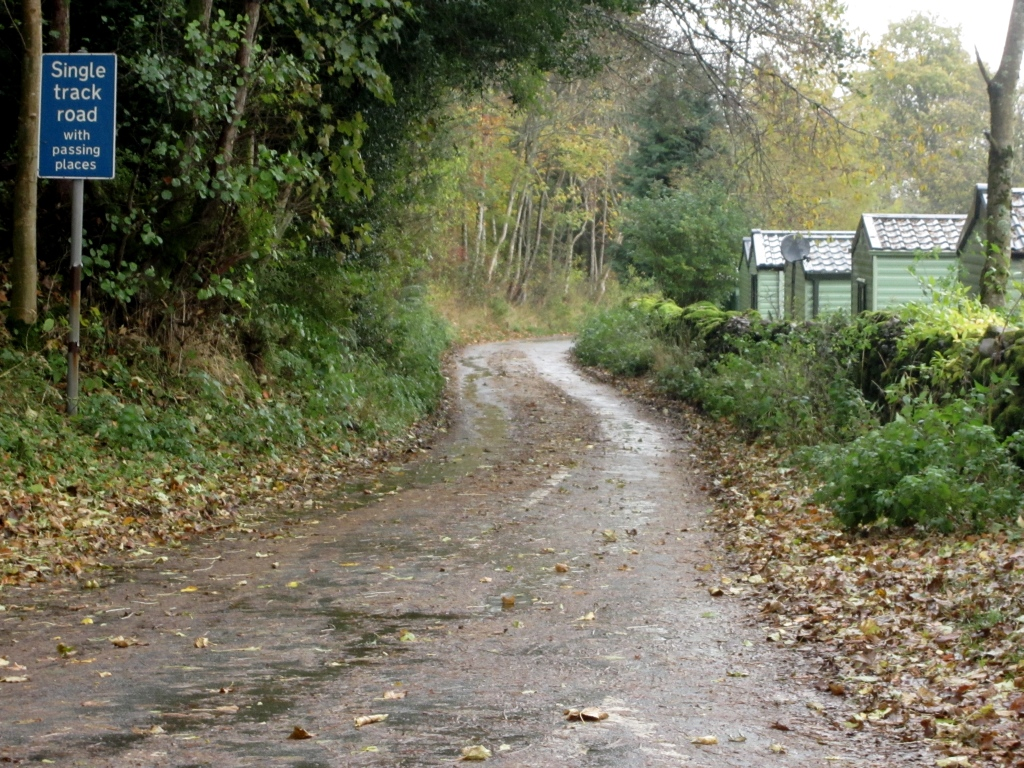
\includegraphics[width=0.488\textwidth,trim=0 65 0 12,clip]{Images/road_example.jpg}%
  }\hfill
  \subfloat[Single-lane warehouse rack corridor with AMR \cite{dematic_radial_amr}.]{%
    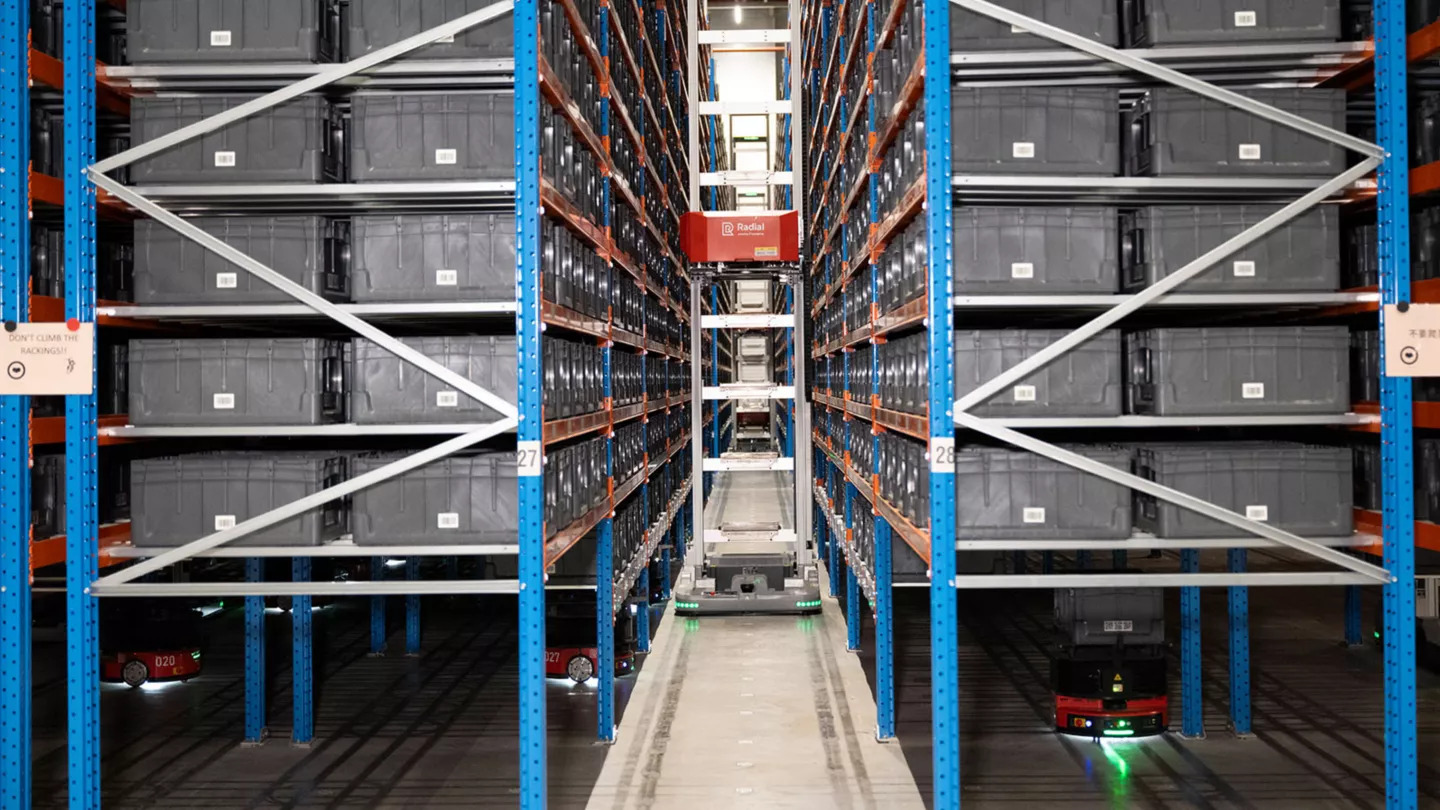
\includegraphics[width=0.488\textwidth]{Images/warehouse_example.jpg}%
  }
  \caption{Representative single-lane environments where two vehicles cannot pass side by side: (a) public road requiring discrete passing places, and (b) high-density warehouse with narrow aisles.}
  \label{fig:narrow_corridor_examples}
\end{figure*}

Given these limitations, an alternative approach is decentralized peer-to-peer negotiation. Rather than avoiding conflicts reactively or resolving them through a central authority (prescriptive collaboration \cite{george2025infrastructure}), encountering robots exchange compact messages over a local broadcast channel and agree on who yields and into which refuge. This retains the infrastructure-free operation of decentralized control while adding coordination to break symmetric deadlocks. 

Prior work spans fixed social laws and traffic rulebooks \cite{kato1992coordinating,shoham1995social,censi2019rulebooks}, market auctions \cite{gerkey2002sold,gautier2022negotiated}, incentive-compatible mechanisms for MAPF and robot prioritization \cite{amir2015mapfauction,das2021omcorp,friedrich2024scalable}, karma economies \cite{censi2019karma,elokda2024karma}, reinforcement-learned give-way policies \cite{bettini2022vmas,bettini2023heterogeneous,park2023hallucination}, and language-model negotiators \cite{marlin2024,gamechat2025,garg2024llm}. Despite this, three research gaps remain \cite{chandra2026social,francis2025principles}, as summarized below.

\begin{enumerate}
\item No shared refuge-and-reversing benchmark across policy families. Corridor give-way studies exist, including MARLIN's single- and two-slot corridors \cite{marlin2024}, VMAS \texttt{give\_way} \cite{vmasgiveway}, and narrow-hallway navigation \cite{park2023hallucination,alghamdi2025opinion}, but each evaluates one or two policy families. None compares rule-based, lock-based, market-based, mechanism-design, and learned policies on the same geometry with nonholonomic turn-and-park maneuvers, asymmetric reverse speeds, and multiple discrete bays (Table~\ref{tab:relwork}). Without such a testbed, competing policies cannot be compared fairly.

\item Siloed assumptions on information, incentives, and channels. Each community resolves conflicts under assumptions that ignore the others'. Rulebooks assume cooperative agents; auctions assume truthful cost estimates; mechanism-design studies assume lossless single-shot games; and communication-tolerant protocols rarely benchmark excess delay against a per-encounter hindsight reference. As a result, no single approach accounts for incentives, channel reliability, and delay together.

\item Unverified 2D-to-3D transfer. Fast 2D simulators make large statistical sweeps cheap but are rarely validated on a real stack. On hardware, wheel slip and acceleration limits alter motion, perception must infer the oncoming robot from noisy Lidar, and messages arrive with jitter rather than in lockstep. These delays are invisible in 2D, so yield decisions and excess-delay results that look sound there may stall or brake late under 3D physics and asynchronous timing.
\end{enumerate}

This paper addresses these gaps with a single refuge-and-reversing benchmark. The benchmark resolves the first gap directly, providing a common testbed that evaluates every policy under realistic turn-and-park maneuvers, asymmetric reverse speeds, and discrete bay placement. It also decomposes the second gap into three strands (information, incentives, and channels) and, for the third, tests which 2D results still hold on a real 3D stack. The study is organized around two architectural layers, namely, a decision mechanism layer determining who yields and into which refuge (RQ1--RQ2), and a distributed execution and embodiment layer governing how robots agree and execute under wireless loss, map errors, and 3D physics (RQ3--RQ4). Together, these layers frame four research questions, detailed next.

\begin{enumerate}
\item RQ1 (Information \& Cost Noise): How much delay do rulebooks, learned lookup tables, and kinematic cost bidding save over reactive backoff and corridor locking, and at what cost-estimation error do heuristic rules catch up to bidding?

\item RQ2 (Incentives \& Fairness): How easily can self-interested robots game unpriced or direct-transfer auctions, what are the budget and collusion trade-offs of Clarke-pivot payments, and how cheaply can historical delay credits balance repeated encounters?

\item RQ3 (Channel Loss \& Map Errors): How does periodic broadcast negotiation survive 99\% packet loss, which safeguards prevent collisions, and how can robots recover from incomplete or obstructed bay maps?

\item RQ4 (Multi-Robot Topologies \& 3D Transfer): What coordination primitives prevent deadlocks in 2-vs.-1 convoys and three-robot T-junctions, and where do 2D kinematic predictions diverge from 3D ROS~2/Gazebo execution?
\end{enumerate}

By addressing these research questions, this paper makes four main contributions.

\begin{enumerate}
\item Benchmark \& Dataset.
A modular ROS~2 benchmark is released that runs the identical 20\,Hz agent state machine in both a fast 2D simulator and 3D Gazebo Harmonic. Every 3D run is seed-paired to a 2D counterpart for direct one-to-one comparison across six narrow-corridor topologies (Fig.~\ref{fig:scen}).

\item Decision-Layer Characterization (RQ1--RQ2).
Reactive, reservation, rulebook, classifier, cost-bidding, and Clarke-pivot policies are benchmarked against the best yield choice across varying corridor geometries and robot speeds. This evaluation quantifies how policies degrade or hold up under log-normal bid noise ($\sigma\in[0,1]$), 27 strategic misreport profiles, and 20-encounter fairness sequences.

\item Protocol Ablation \& Map-Resilience Primitives (RQ3).
Three communication safeguards are ablated across 5,760 episodes under 90--99\% packet loss and 2--8\,s latency. The ablation records zero collisions in every configuration, even with all three radio safeguards disabled (indicating that local Lidar stopping margins and randomized exit timers, rather than the radio safeguards, prevent collisions), while the \texttt{commit} handshake adds 3--4\,s of waiting without reducing deadlocks. A zero-overhead map-recovery primitive piggybacks each robot's known bay list onto existing \texttt{BID} messages, restoring shared bay awareness under incomplete maps without extra packets.

\item Multi-Robot Extensions \& Gazebo Audit (RQ4).
Two-robot negotiation is extended to 2-vs.-1 convoys and three-robot T-junctions using follower backoff (\texttt{make\_room}), combined convoy bidding (\gb), and junction staging (\texttt{goal\_wait}), revealing why simply adding individual robot costs underestimates convoy yield time when the follower must reverse clear before the leader can back up. Across 496 seed-paired Gazebo runs, 2D and 3D select the same yielding robot in $97.0\%$ of encounters and match corridor excess delays within $1.0$~s, with the remaining differences traced to 3D Lidar detection range and three-robot junction timing.
\end{enumerate}

The remainder of this paper reviews related work (Sec.~\ref{sec:rel}), formulates the physical encounter and protocol architecture (Sec.~\ref{sec:bench}), defines the policy families and mechanism equations (Sec.~\ref{sec:pol}), details the experimental design and statistical conventions (Sec.~\ref{sec:exp}), presents empirical findings for RQ1--RQ4 (Secs.~\ref{sec:rq1}--\ref{sec:rq4}), synthesizes practitioner guidelines and limitations (Sec.~\ref{sec:disc}), and concludes (Sec.~\ref{sec:conc}).
\section{Related Work}\label{sec:rel}
\vspace{-0.2cm}
Resolving head-on encounters in narrow, bay-equipped corridors draws on several research threads that have largely developed in isolation. This section reviews four strands, covering (i)~reactive local planners and their deadlock-breaking extensions, (ii)~centralized traffic management, zone control, and multi-agent path finding (MAPF), (iii)~decentralized negotiation and mechanism design, including karma-based credit economies, and (iv)~learned negotiators and the benchmarks used to evaluate multi-robot navigation. For each, this section identifies the assumptions that break down when a corridor admits only one robot at a time and yielding requires a costly reverse maneuver into a discrete pull-in bay.

\subsection{Deadlock in Symmetric and Constrained Navigation}
Local reactive planners such as the Dynamic Window Approach \cite{fox1997dwa}, Velocity Obstacles \cite{fiorini1998motion}, RVO/ORCA \cite{vandenberg2011orca}, and decentralized CBFs \cite{wang2017safety} achieve scalable collision avoidance in open spaces, yet stall in symmetric head-on bottlenecks where geometric velocity cones or barrier gradients cancel \cite{grover2023before}. Grover et al. \cite{grover2023before} formally characterize the equilibrium sets of CBF deadlocks; Zheng and Li \cite{zheng2023deadlock} perturb nonholonomic controls to escape symmetric stalls; Dergachev and Yakovlev \cite{dergachev2021distributed} switch stalled ORCA clusters to local MAPF; and Chandra et al. \cite{chandra2025deadlock,chandra2026social} cast doorway and hallway encounters as ``social mini-games'' resolved via discrete-time CBFs. However, those methods only break deadlocks in spaces wide enough for robots to pass by adjusting speed or shifting slightly to the side. When a corridor is narrower than two robot bodies, neither robot can pass until one selects a discrete pull-in bay behind it, reverses into that bay, parks clear of the main lane, and waits for the oncoming robot to clear the aisle.

\subsection{Centralized Traffic Management, Zone Control, and MAPF}
In structured warehouses, multi-robot coordination is predominantly centralized \cite{fragapane2021planning}. Classical Automated Ground Vehicle (AGV) zone control partitions aisles into mutually exclusive blocks governed by Petri nets or geometric locks \cite{fanti2002event}, a paradigm directly represented by the first-come \texttt{reservation} baseline in this work. Graph-based MAPF solvers, including CBS \cite{sharon2015cbs}, PIBT \cite{okumura2022pibt}, LaCAM \cite{okumura2023lacam}, safe-interval path planning (SIPP) \cite{phillips2011sipp}, and narrow-corridor extensions \cite{experience2024narrow,macga2025}, treat pull-in bays as graph vertices, while kinodynamic planners \cite{wen2022clmapf,dbecbs2025} and industrial traffic frameworks such as Open-RMF \cite{openrmf}, VDA 5050 \cite{vda5050}, and hierarchical zone managers \cite{hiertraffic2023} arbitrate schedules centrally. Precedence-preserving execution protocols \cite{cap2016provably,mannucci2019provably} further maintain safety under timing delays or unreliable links once a central priority graph is fixed. Unlike the above-mentioned approaches, this paper studies fully decentralized encounter resolution without pre-computed joint schedules, and explicitly penalizes the slower reverse kinematics that symmetric graph edge weights ignore.

\subsection{Decentralized Negotiation, Mechanism Design, and Karma}
Decentralized conflict resolution through explicit rules and messaging dates back to Kato et al. \cite{kato1992coordinating} and Shoham and Tennenholtz's offline social laws \cite{shoham1995social}, alongside local path-negotiation protocols \cite{purwin2008theory} and connected-vehicle bottleneck etiquette \cite{bottleneckiv2023}. Market-based robotics \cite{gerkey2002sold} allocates tasks and intersections \cite{dresner2008multiagent} via cost bids, and Gautier et al. \cite{gautier2022negotiated} negotiate path conflicts among non-cooperative robots. Yet simple ``lower-bid-yields'' or direct side-payment schemes assume honest reporting. Algorithmic mechanism design \cite{nisan2001algorithmic} via Vickrey--Clarke--Groves (VCG) pivot payments \cite{clarke1971multipart} makes truthful cost reporting a dominant strategy, subject to the classical Green--Laffont and Myerson--Satterthwaite impossibility results prohibiting simultaneous efficiency, truthfulness, and strict budget balance \cite{green1977characterization}. For repeated right-of-way interactions where monetary billing is undesirable, Censi et al. \cite{censi2019karma} and Elokda et al. \cite{elokda2024karma} introduce self-contained ``karma'' credit economies. Meanwhile, communication-impairment surveys and delay-tolerant protocols \cite{commfail2021,gielis2022critical} highlight packet drops and staleness as critical deployment bottlenecks, motivating the empirical safeguard ablation at up to 99\% loss presented here.

\subsection{Learned Negotiators and Multi-Robot Benchmarks}
Deep multi-agent reinforcement learning (MARL) has been widely applied to decentralized collision avoidance \cite{chen2017cadrl,yu2022mappo} and constrained corridor give-way tasks such as VMAS \texttt{give\_way} \cite{vmasgiveway,bettini2023heterogeneous} and perceptual obstacle hallucination \cite{park2023hallucination}. Recent works also explore large language models (LLMs) for MARL reward/prior guidance in slotted corridors (MARLIN \cite{marlin2024}), multi-agent doorway dialogue (GameChat \cite{gamechat2025}), and centralized deadlock recovery \cite{garg2024llm}. Standardized navigation testbeds such as BARN \cite{xiao2022barn} and SocNavBench \cite{francis2025principles} have accelerated reproducible evaluation in cluttered and social spaces, while Gazebo \cite{gazebosim} provides high-fidelity ROS~2 physics. However, no existing benchmark evaluates classical heuristics, zone locks, kinematic auctions, VCG mechanisms, and learned lookup policies side by side under unified nonholonomic bay geometry, communication stress, and seed-paired 2D-to-Gazebo validation.


\section{Problem Formulation}\label{sec:problem}\label{sec:bench}

\begin{figure*}[!t]
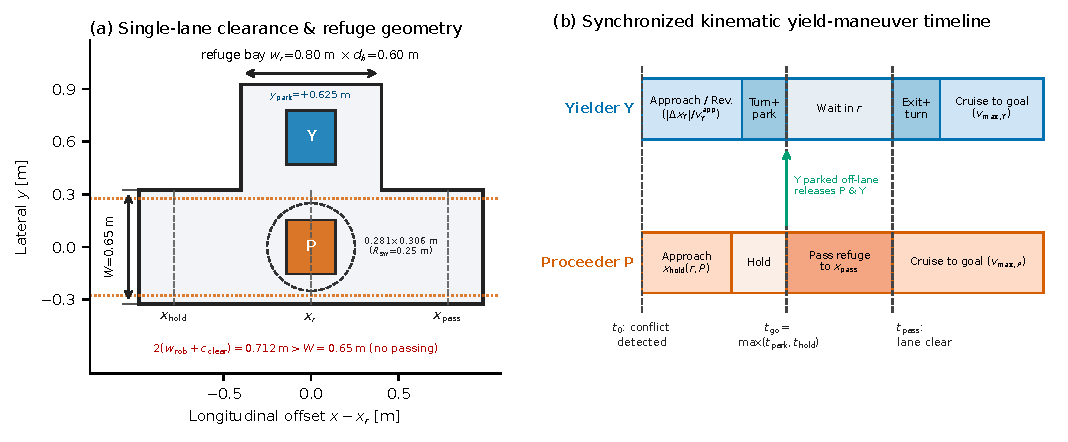
\includegraphics[width=1\textwidth]{Images/problem_formulation.pdf}
\caption{Physical and kinematic formulation of a narrow-corridor encounter. (a) Cross-sectional clearance constraint~\eqref{eq:width_constraint}: two robots of width $w_{\mathrm{rob}}=0.306$\,m with clearance $c_{\mathrm{clear}}=0.05$\,m require $0.712$\,m laterally and cannot pass side by side within corridor width $W=0.65$\,m unless yielder $Y$ parks at lateral offset $y_{\mathrm{park},r}$ inside refuge $r$. (b) Synchronized kinematic yield-maneuver timeline~\eqref{eq:geom}--\eqref{eq:timeline} showing hold point $x_{\mathrm{hold}}(r,P)$, clearance point $x_{\mathrm{pass}}(r,P)$, and phase synchronization instants $t_{\mathrm{park}}$, $t_{\mathrm{go}}$, and $t_{\mathrm{pass}}$.}
\label{fig:formulation}
\end{figure*}

This paper considers a decentralized right-of-way resolution problem in which AMRs traverse a single-lane corridor that is physically too narrow for side-by-side passage. When two or more robots travel in opposing directions, at least one must temporarily vacate the main travel lane by maneuvering into a discrete off-lane refuge so that oncoming traffic can pass. Table~\ref{tab:nomenclature} summarizes the key notation used across the problem formulation and negotiation mechanisms, while fixed physical parameters are listed in Table~\ref{tab:params}.

\begin{table}[!t]\centering
\caption{Summary of Principal Mathematical Notation.}
\label{tab:nomenclature}
{\footnotesize\renewcommand{\arraystretch}{1.28}\setlength{\tabcolsep}{3.5pt}\medmuskip=2mu\thickmuskip=3mu
\resizebox{\columnwidth}{!}{\begin{tabular}{@{}ll@{}}\toprule
Symbol & Definition \\\midrule
\multicolumn{2}{@{}l}{\emph{Sets, Indices, and Refuges}} \\\addlinespace[2pt]
$i \in \{A, B\}$; $Y, P$ & Robot index; candidate yielder and proceeder \\
$\mathcal{G}_Y, \mathcal{G}_P$ & Yielding and proceeding convoy robot groups \\
$\mathcal{R},\, r \in \mathcal{R}$ & Discrete refuge set and individual refuge index \\
$x_r, w_r, y_{\mathrm{park},r}$ & Refuge entry coordinate, width, and parking offset \\
$\mathcal{F}(Y,P),\, r^\ast$ & Feasible refuge set for $(Y,P)$ and delay-optimal refuge \\\addlinespace[2pt]\midrule
\multicolumn{2}{@{}l}{\emph{Robot State and Feasibility (Eqs.~\eqref{eq:width_constraint}--\eqref{eq:geom})}} \\\addlinespace[2pt]
$x_i, v_i, s_i \in \{\pm 1\}$ & Longitudinal position, speed, and travel direction \\
$x_{\mathrm{goal},i}, t_{\mathrm{enter},i}$ & Goal coordinate and corridor entry timestamp \\
$u_i \ge 1,\, l_i \in \{0,1\}$ & Task urgency weight and binary payload flag \\
$v_{\max,i}, v_{\mathrm{rev},i}, v_Y^{\mathrm{app}}$ & Forward, reverse, and refuge-approach speed limits \\
$x_{\mathrm{stop}}, x_{\mathrm{hold}}, x_{\mathrm{pass}}$ & Proceeder braking, hold, and refuge-clearance lines \\\addlinespace[2pt]\midrule
\multicolumn{2}{@{}l}{\emph{Maneuver Timeline and Delay (Eqs.~\eqref{eq:timeline}--\eqref{eq:social_obj})}} \\\addlinespace[2pt]
$T_i^{\mathrm{free}}, t_{\mathrm{turn}}$ & Free-flow travel time and $90^\circ$ bay-turn duration \\
$t_{\mathrm{park}}, t_{\mathrm{hold}}, t_{\mathrm{go}}, t_{\mathrm{pass}}$ & Park, hold-arrival, proceeder-release, and clearance times \\
$T_i(r),\, d_i(r)$ & Total arrival time and encounter delay via refuge $r$ \\
$C_{\mathrm{soc}}(Y,r)$ & Pairwise urgency-weighted social delay cost \\\addlinespace[2pt]\midrule
\multicolumn{2}{@{}l}{\emph{Bidding, Incentives, and Evaluation (Eqs.~\eqref{eq:costbid}--\eqref{eq:excess})}} \\\addlinespace[2pt]
$\tilde{c}_Y,\, \sigma,\, \epsilon_Y$ & Noisy social-cost bid, log-normal noise scale, and draw \\
$C_{\mathrm{grp}}(\mathcal{G}_Y,\mathcal{G}_P)$ & Side-level convoy group-bidding social cost \\
$o \in \{A,B\},\, o^\ast$ & Candidate yield outcome and mechanism-selected outcome \\
$b_i(o),\, p_i$ & Reported delay cost for outcome $o$ and Clarke VCG payment \\
$D_{i,t}^{\mathrm{cum}},\, \lambda$ & Cumulative delay through encounter $t$ and fairness weight \\
$D_\pi^{(k)},\, \Delta_\pi$ & Episode delay on encounter $k$ and paired excess delay \\\bottomrule
\end{tabular}}}
\end{table}

\subsection{Spatial Domain and Single-Lane Passing Constraint}
The environment is a straight corridor of length $L$ and width $W$ centered along the $x$-axis ($y = 0$), connecting two open staging rooms at $x \le 0$ and $x \ge L$ (Fig.~\ref{fig:formulation}a). Distributed along the corridor walls and inside both end rooms is a discrete set of off-lane refuges $\mathcal{R}$ (pull-in bays and end-room parking zones). Each refuge $r \in \mathcal{R}$ is defined by its longitudinal entry coordinate $x_r$, opening width $w_r$, and lateral parking offset $y_{\mathrm{park},r}$ required to clear the main lane. 

Each robot has chassis width $w_{\mathrm{rob}}$, rotational swept radius $R_{\mathrm{sw}}$, and required safety margin $c_{\mathrm{clear}}$ from walls and other robots. While inside the corridor, robots track the centerline $y = 0$. Side-by-side passing is physically impossible because the combined width of two robots and their safety margins exceeds the corridor width, such that

\begin{equation}
2\bigl(w_{\mathrm{rob}} + c_{\mathrm{clear}}\bigr) > W.
\label{eq:width_constraint}
\end{equation}
Consequently, two opposing robots $A$ and $B$ cannot pass each other inside the corridor unless one robot pulls into a refuge $r \in \mathcal{R}$ while the other drives past $x_r$.

\subsection{Robot State and Asymmetric Kinematics}
Each robot $i \in \{A, B\}$ is characterized by its longitudinal position $x_i$, speed $v_i$, travel direction $s_i \in \{+1, -1\}$ (toward $+x$ or $-x$), and goal coordinate $x_{\mathrm{goal},i}$, along with three task attributes comprising corridor entry time $t_{\mathrm{enter},i}$, urgency weight $u_i \ge 1$, and binary payload flag $l_i \in \{0, 1\}$.
Robots follow unicycle kinematics with maximum linear acceleration $a_{\max,i}$, maximum turn rate $\omega_{\max,i}$, and asymmetric forward and reverse speed limits satisfying

\begin{equation}
-v_{\mathrm{rev},i} \le v_i \le v_{\max,i}, \qquad 0 < v_{\mathrm{rev},i} < v_{\max,i}.
\label{eq:speed_bounds}
\end{equation}

Because reversing is slower than driving forward ($v_{\mathrm{rev},i} < v_{\max,i}$) and entering or exiting a bay requires two $90^\circ$ turns, backing into a refuge behind a robot takes significantly longer than pulling into one ahead.

\subsection{Refuge Feasibility Constraints}
When two opposing robots $A$ and $B$ meet, a candidate resolution assigns one robot as the \emph{yielder} $Y \in \{A, B\}$, the other as the \emph{proceeder} $P$, and selects a target refuge $r \in \mathcal{R}$ for $Y$.
For $P$ to pass safely while $Y$ is parked in refuge $r$, three longitudinal coordinates along the centerline govern the maneuver (Fig.~\ref{fig:formulation}a), namely, $P$'s minimum braking coordinate $x_{\mathrm{stop}}$, the hold line $x_{\mathrm{hold}}$ where $P$ must wait if $Y$ is not yet parked, and the clearance line $x_{\mathrm{pass}}$ where $P$ has fully passed the refuge, defined as

\begin{equation}
\begin{aligned}
x_{\mathrm{stop}} &= x_P + s_P \frac{v_P^2}{2 a_{\max,P}}, \\
x_{\mathrm{hold}} &= x_r - s_P \Bigl(\frac{w_r}{2} + R_{\mathrm{sw}} + c_{\mathrm{clear}}\Bigr), \\
x_{\mathrm{pass}} &= x_r + s_P \Bigl(\frac{w_r}{2} + R_{\mathrm{sw}} + c_{\mathrm{clear}}\Bigr).
\end{aligned}
\label{eq:geom}
\end{equation}

A refuge $r \in \mathcal{R}$ belongs to the \emph{feasible refuge set} $\mathcal{F}(Y, P)$ if it is unobstructed and satisfies three conditions along each robot's travel direction, stated below.
\begin{enumerate}
\item \emph{Braking margin:} $P$ can stop before the hold line, $s_P(x_{\mathrm{hold}} - x_{\mathrm{stop}}) \ge 0$;
\item \emph{Proceeder progression:} $P$'s goal lies beyond the clearance line, $s_P(x_{\mathrm{goal},P} - x_{\mathrm{pass}}) \ge 0$; and
\item \emph{Yielder progression:} $Y$'s goal lies beyond the refuge entry, $s_Y(x_{\mathrm{goal},Y} - x_r) \ge 0$.
\end{enumerate}

\subsection{Maneuver Timeline and Delay Model}
Without opposing traffic, robot $i$ cruises directly to its goal in free-flow time $T_i^{\mathrm{free}} = |x_{\mathrm{goal},i} - x_i| / v_{\max,i}$.
When yielder $Y$ pulls into a feasible refuge $r \in \mathcal{F}(Y, P)$, the maneuver unfolds in four sequential stages (Fig.~\ref{fig:formulation}b), summarized below.
\begin{enumerate}
\item \emph{Yielder parks ($t_{\mathrm{park}}$):} $Y$ travels to $x_r$ at speed $v_Y^{\mathrm{app}}$ ($v_{\mathrm{rev},Y}$ if reversing, $v_{\max,Y}$ if driving forward), rotates $90^\circ$ in time $t_{\mathrm{turn}} = (\pi/2)/(0.8\,\omega_{\max,Y})$, and pulls into $y_{\mathrm{park},r}$.
\item \emph{Proceeder holds ($t_{\mathrm{go}}$):} $P$ reaches the hold line at $t_{\mathrm{hold}} = |x_{\mathrm{hold}} - x_P| / v_{\max,P}$ and waits if $Y$ is not yet parked, departing at $t_{\mathrm{go}} = \max(t_{\mathrm{park}},\, t_{\mathrm{hold}})$.
\item \emph{Proceeder passes ($t_{\mathrm{pass}}$):} $P$ drives past the refuge to clear $x_{\mathrm{pass}}$, then continues to $x_{\mathrm{goal},P}$.
\item \emph{Yielder resumes ($T_Y$):} Once $P$ clears $x_{\mathrm{pass}}$, $Y$ reverses out of the bay, rotates $90^\circ$ back onto the centerline, and drives to $x_{\mathrm{goal},Y}$.
\end{enumerate}
The resulting milestone times ($t_{\mathrm{park}}, t_{\mathrm{pass}}$) and total arrival times ($T_Y, T_P$) are given by
\begin{equation}
\begin{aligned}
t_{\mathrm{park}} &= \frac{|x_r - x_Y|}{v_Y^{\mathrm{app}}} + t_{\mathrm{turn}} + \frac{|y_{\mathrm{park},r}|}{v_{\max,Y}}, \\
t_{\mathrm{pass}} &= \max(t_{\mathrm{park}},\, t_{\mathrm{hold}}) + \frac{|x_{\mathrm{pass}} - x_{\mathrm{hold}}|}{v_{\max,P}}, \\
T_Y(r) &= t_{\mathrm{pass}} + \frac{|y_{\mathrm{park},r}|}{v_{\mathrm{rev},Y}} + t_{\mathrm{turn}} + \frac{|x_{\mathrm{goal},Y} - x_r|}{v_{\max,Y}}, \\
T_P(r) &= t_{\mathrm{pass}} + \frac{|x_{\mathrm{goal},P} - x_{\mathrm{pass}}|}{v_{\max,P}}.
\end{aligned}
\label{eq:timeline}
\end{equation}
Each robot's predicted encounter delay is the extra time incurred above free flow, defined as
\begin{equation}
d_i(r) = T_i(r) - T_i^{\mathrm{free}}, \qquad i \in \{Y, P\},
\label{eq:delay_def}
\end{equation}
and the optimal refuge for candidate yielder $Y$ is the feasible refuge that minimizes combined delay, $r^\ast(Y, P) = \arg\min_{r \in \mathcal{F}(Y, P)} [d_Y(r) + d_P(r)]$ (breaking ties by closest $|x_r - x_Y|$).

\subsection{Optimization Objectives and Operational Constraints}
Ideally, when two opposing robots $A$ and $B$ meet with full map knowledge and honest communication, the goal is to choose the yielder $Y \in \{A, B\}$ and feasible refuge $r \in \mathcal{F}(Y, P)$ that minimize total urgency-weighted delay according to
\begin{equation}
\min_{Y \in \{A, B\},\; r \in \mathcal{F}(Y, P)} \; C_{\mathrm{soc}}(Y, r) = u_Y d_Y(r) + u_P d_P(r).
\label{eq:social_obj}
\end{equation}

In real warehouse deployments, however, solving~\eqref{eq:social_obj} without a central traffic controller faces four practical challenges that motivate the four research questions below.
\begin{enumerate}
\item Imperfect Information and Cost Noise (RQ1): Robots rarely know exact future travel times; they must decide using noisy delay predictions, simplified priority rules, or learned lookup policies that may not generalize to new corridor layouts.
\item Self-Interested Bidding vs.\ Long-Run Fairness (RQ2): In multi-vendor fleets, a self-interested robot can exaggerate its delay cost to avoid yielding unless truth-telling is enforced via mechanism payments. Conversely, in a cooperative fleet across repeated encounters, static priority rules repeatedly delay the same robot, requiring a trade-off between single-encounter efficiency and cumulative fairness~\cite{jain1984fairness}.
\item Lossy Communication and Incomplete Maps (RQ3): Robots negotiate over wireless links subject to packet drops and latency, and may only know a subset of refuges discovered within local sensor range or blocked by unmapped obstacles.
\item Multi-Robot Coupling and 3D Physical Transfer (RQ4): Pairwise corridor negotiation must scale to three-robot encounters (convoys and T-junctions where a third robot can block a yielder) and transfer reliably from fast 2D kinematic models to 3D rigid-body physics and Lidar perception.
\end{enumerate}

\section{Experimental Design and Methodology}\label{sec:exp}
To evaluate how decentralized negotiation mechanisms perform under the physical, informational, strategic, and communication constraints formulated in Section~\ref{sec:problem}, this section develops a modular negotiation protocol, a nine-policy benchmark taxonomy, and a reproducible dual-simulator experimental suite, organized around RQ1--RQ4.

\subsection{Decentralized Negotiation Protocol and Safeguards}\label{sec:proto}
All communicating policies execute inside a shared five-mode agent state machine (\texttt{CRUISE}, \texttt{NEGOTIATE}, \texttt{YIELD}, \texttt{PROCEED}, \texttt{DONE}) stepped at $20$\,Hz ($\Delta t = 0.05$\,s; Fig.~\ref{fig:proto}a).

\begin{figure*}[!t]\centering
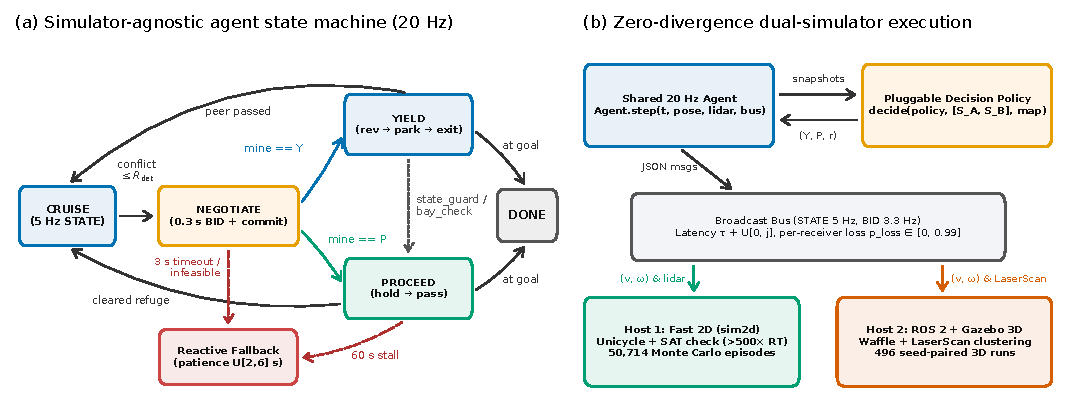
\includegraphics[width=1\textwidth]{Images/protocol.pdf}
\caption{Decentralized negotiation protocol and dual-simulator execution architecture. (a) Simulator-agnostic $20$\,Hz agent state machine showing nominal transitions (solid), timeout/infeasibility reactive fallbacks (dashed red), and lossy-channel yield-abort guards (dotted gray). (b) Zero-code-divergence execution architecture connecting the shared $20$\,Hz \texttt{Agent} controller and pluggable decision policy to both the fast 2D unicycle simulator (\texttt{sim2d}) and 3D ROS~2 Jazzy / Gazebo Harmonic.}
\label{fig:proto}
\end{figure*}

\subsubsection{Conflict Detection and Deterministic Snapshot Resolution}
While in \texttt{CRUISE}, robots broadcast 5\,Hz \texttt{STATE} beacons containing their pose, velocity, control mode, and corridor entry time (considered fresh for 1.0\,s). A conflict is triggered when a peer's beacon indicates an opposing robot within $R_{\mathrm{det}} = 6.0$\,m. Setting $R_{\mathrm{det}}$ beyond the 3.5\,m Lidar range ensures negotiation starts before either vehicle drives past a usable refuge.
Upon detection, each robot freezes its state into a kinematic \texttt{Snapshot} $S_i$ (pose, speed bounds, urgency, and payload status) and broadcasts it in a \texttt{BID} packet retransmitted every $0.3$\,s. Because each policy is a deterministic function of the sorted snapshot pair $(S_A, S_B)$ and the shared map, both robots independently compute the exact same \texttt{(yielder, proceeder, refuge)} assignment locally without requiring an extra handshake message.

\subsubsection{Lossy-Channel Safeguards and Liveness Fallbacks} 
Under severe packet drops or latency, robots may receive delayed messages and compute conflicting decisions. To prevent inconsistent execution, the protocol implements three switchable safeguards.
\begin{itemize}
\item \emph{Commit handshake (\texttt{commit}):} Robots attach their planned decision to outgoing \texttt{BID}s and wait for mutual confirmation. If decisions disagree, the lower-ID robot's choice takes precedence; unconfirmed decisions expire after 3.0\,s.
\item \emph{State guard (\texttt{state\_guard}):} A yielding robot monitors incoming peer \texttt{STATE} beacons and aborts its maneuver (switching to \texttt{PROCEED}) if the peer is also yielding to it or heading into the same bay.
\item \emph{Lidar bay check (\texttt{bay\_check}):} Bays with Lidar returns within 0.45\,m of the parking spot are treated as occupied during planning. If an en-route yielder detects a peer inside its target bay, it aborts and proceeds.
\end{itemize}
During execution, a proceeding robot advances only once \texttt{STATE} beacons or Lidar confirm the yielder is off-lane (renegotiating if the yielder continues cruising toward it). Similarly, a parked yielder exits once peer \texttt{STATE} confirms passage. If packet loss renders \texttt{STATE} stale, the yielder exits when Lidar confirms the peer has passed, or after a randomized hold $U[6,12]$\,s once the lane is clear.
To guarantee liveness under communication blackouts or deadlocks, robots fall back to reactive backoff when (i)~no peer \texttt{BID} arrives within $\tau_{\mathrm{neg}} = 3.0$\,s, (ii)~a proceeding robot stalls for $\tau_{\mathrm{proc}} = 60.0$\,s, or (iii)~neither robot has a feasible refuge ($\mathcal{F}=\emptyset$), triggering a 10.0\,s backoff. Receiving a valid peer \texttt{BID} at any time immediately resumes negotiation.

\subsubsection{Map-Uncertainty and Multi-Robot Extensions} 
Five protocol extensions address incomplete maps and multi-robot interactions. For map uncertainty, three extensions are included, namely, 
(i)~\texttt{share\_map} attaches known bay IDs to every \texttt{BID} so peers merge their maps before planning; 
(ii)~\texttt{explore} starts robots knowing only end rooms and discovers bays via Lidar within 3.5\,m (optionally gating map exchange on visual peer detection via \texttt{share\_on\_detect}, or pausing decisions up to 15.0\,s to await peer maps via \texttt{hold\_for\_map}); and 
(iii)~\texttt{refuge\_blocked} cross-checks Lidar returns inside bays against peer \texttt{STATE} beacons, broadcasting unmapped physical obstacles as blocked rather than mistaking them for parked robots. 
For multi-robot topologies, two rules are added, namely, 
(iv)~convoy \texttt{make\_room} instructs a trailing follower to back into an upstream bay if it blocks its reversing leader; and 
(v)~T-junction \texttt{goal\_wait} directs a robot whose branch destination is occupied to wait off-lane in an upstream bay rather than blocking the main corridor.

\subsection{Evaluated Coordination Policies}\label{sec:pol}
Table~\ref{tab:taxonomy} summarizes the nine policies evaluated across the benchmark studies. All negotiating policies map the frozen snapshot pair $(S_A, S_B)$ to a yielder $Y \in \{A, B\}$ and feasible refuge $r \in \mathcal{F}(Y, P)$.

\subsubsection{Non-Communicating, Lock, and Heuristic Rulebook Policies}
\texttt{reactive} (R) uses no communication; when Lidar detects an oncoming peer within braking distance, the robot stops, waits a random patience duration $U[2,6]$\,s to break symmetry, and reverses into the nearest refuge behind it if still blocked.
\texttt{reservation} (S) emulates first-come, first-served (FCFS) industrial zone control~\cite{fanti2002event} via \texttt{STATE} beacons; a robot outside the corridor ($[0,L]$) waits in its staging room whenever an opposing vehicle is already inside the aisle (falling back to \texttt{rules\_default} if both enter simultaneously).
\texttt{fixed\_priority} (F) is a static rule where the higher-ID robot always yields into its best feasible refuge $r^\ast$ unless no refuge is available ($\mathcal{F}=\emptyset$).
\texttt{rules\_default} (D) applies an ordered six-tier etiquette~\cite{kato1992coordinating,highwaycode} evaluated sequentially, checking 
(1)~refuge availability (if only one robot has a feasible refuge $\mathcal{F} \neq \emptyset$, it yields); 
(2)~task urgency (if $|u_A - u_B| \ge 0.5$, the less urgent robot yields); 
(3)~payload status (an unloaded robot yields to a loaded one); 
(4)~corridor seniority (the later entrant by $\ge 1.0$\,s yields); 
(5)~nearby refuge (if only one robot has a refuge within 2.0\,m behind it, it yields); and 
(6)~lower-ID tie-break. 
\texttt{rules\_proximity} (P) modifies this hierarchy by prioritizing geometry ahead of seniority, such that whichever robot is closer to its feasible refuge (by $\ge 0.1$\,m) yields immediately after checking payload.

\begin{table*}[!t]\centering
\caption{Taxonomy of benchmarked corridor coordination policies across communication, information inputs, model assumptions, and strategic properties.}
\label{tab:taxonomy}
{\footnotesize\setlength{\tabcolsep}{2.9pt}
\begin{tabular}{@{}llcccc>{\raggedright\arraybackslash}p{0.190\textwidth}@{}}\toprule
Policy (Code) & Family & Comms & State Inputs Used & Motion Model & Incentive Prop. & Multi-Robot / Map Scope \\\midrule
\texttt{reactive} (R) & Local sensor backoff & None & $3.5$\,m Lidar proximity & None & N/A & Pairwise/local; patience $U[2,6]$\,s \\
\texttt{reservation} (S) & Corridor mutex lock & \texttt{STATE} & Occupancy, $t_{\mathrm{enter}}$ & None & First-in wins & Corridor FCFS; rulebook inside-tie \\
\texttt{fixed\_priority} (F) & Static social law & \texttt{STATE}+\texttt{BID} & Robot ID, feasibility & Feasibility only & Non-manipulable$^\dagger$ & Pairwise + \texttt{make\_room} / \texttt{goal\_wait} \\
\texttt{rules\_default} (D) & Lexicographic rules & \texttt{STATE}+\texttt{BID} & $u_i$, load, $t_{\mathrm{enter}}$, bay $\le 2$\,m & Feasibility only & Non-manipulable$^\dagger$ & Ordered 6-rule industrial etiquette \\
\texttt{rules\_proximity} (P) & Geometric rulebook & \texttt{STATE}+\texttt{BID} & Nearest-bay $|x_r - x_i|$, D & Refuge distance & Pose-dependent & Closest-refuge ahead of seniority \\
\texttt{learned} (L) & Tabular classifier & \texttt{STATE}+\texttt{BID} & Binned bay dist., $u_i$, load & Offline sim table & Co-op assumed & 93 states; unseen $\to$ fixed priority \\
\cb\ (C) & Kinematic auction & \texttt{STATE}+\texttt{BID} & Full \texttt{Snapshot}, $u_i$ & Constant-speed & Manipulable & Pairwise social-cost minimization \\
\gb\ (G) & Convoy auction & \texttt{STATE}+\texttt{BID} & Group \texttt{Snapshot}s & Side-level sum & Co-op assumed & Distinct bays across convoy group \\
\texttt{clarke} (V) & VCG mechanism & \texttt{STATE}+\texttt{BID} & Cost vectors $b_i(o)$ & Constant-speed & DSIC (unilat.)$^\ddagger$ & Externality payment to fleet bank \\\bottomrule
\end{tabular}}\\[2pt]
{\footnotesize $^\dagger$Non-manipulable with respect to cost bids; physical state claims ($u_i$, load, known bays) are assumed authentic. $^\ddagger$Dominant-strategy incentive compatible for unilateral cost scaling under the shared kinematic model; runs a budget surplus and does not prevent joint shading or bay-set omission.}
\end{table*}

\subsubsection{Kinematic Cost Bidding (\cb) and Convoy Group Bidding (\gb)}
Under \cb\ (C), robots select the yielder that minimizes predicted urgency-weighted social delay using equation \eqref{eq:timeline}. Each candidate yielder $Y \in \{A, B\}$ evaluates

\begin{equation}
\begin{aligned}
\tilde{c}_Y &= \bigl(u_Y d_Y(r^\ast) + u_P d_P(r^\ast)\bigr)\exp(\sigma \epsilon_Y), \\
Y^\ast &= \arg\min_{Y\in\{A,B\}} \tilde{c}_Y,
\end{aligned}
\label{eq:costbid}
\end{equation}

where $\epsilon_Y \sim \mathcal{N}(0,1)$ introduces log-normal estimation noise (with $\sigma = 0$ by default, and $\sigma > 0$ in study \texttt{S7}), and $\tilde{c}_Y = \infty$ if no refuge is feasible ($\mathcal{F}=\emptyset$). The robot with the lower bid yields.
For multi-robot convoys (yielding group $\mathcal{G}_Y$ vs.\ proceeding group $\mathcal{G}_P$), \gb\ (G) attaches follower snapshots to the leader's \texttt{BID}. It assigns distinct bays greedily across yielding members (sharing end rooms if necessary) and computes a side-level social cost as

\begin{equation}
\begin{aligned}
C_{\mathrm{grp}}(\mathcal{G}_Y,\mathcal{G}_P) &= \sum_{y\in\mathcal{G}_Y} u_y d_y(r_y^\ast) \\
&\quad + \Bigl(\max_{f\in\mathcal{G}_P\setminus\{P\}}\frac{|x_f-x_P|}{v_{\max,f}}\Bigr)\!\sum_{y\in\mathcal{G}_Y} u_y \\
&\quad + \Bigl(\max_{y\in\mathcal{G}_Y} d_{P,y}(r_y^\ast)\Bigr)\!\sum_{p\in\mathcal{G}_P} u_p.
\end{aligned}
\label{eq:groupbid}
\end{equation}

The three terms in Eq.~\eqref{eq:groupbid} represent (i)~the cumulative yield delays of group $\mathcal{G}_Y$, (ii)~the yielding group's wait while proceeding followers pass, and (iii)~the proceeding group's delay while the slowest yielder parks.
Crucially, Eq.~\eqref{eq:groupbid} sums member yield delays additively. Because it assumes concurrent maneuvering rather than modeling the \emph{serial} wait required for trailing followers to reverse via \texttt{make\_room}, \gb\ underestimates the true cost of yielding an entire convoy when the oncoming lone vehicle has high urgency (Sec.~\ref{sec:rq4}).

\subsubsection{Clarke-Pivot (VCG) Mechanism and Repeated Fairness Credit}
Simple cost bidding is vulnerable to strategic manipulation, as robots can artificially inflate bids to avoid yielding, while naive direct side-payments incentivize under-reporting. To enforce truthful reporting, \texttt{clarke} (V)~\cite{clarke1971multipart} implements a Vickrey--Clarke--Groves (VCG) pivot mechanism. Each robot reports its predicted delay cost $b_i(o)$ for both possible outcomes $o \in \{A, B\}$ (where $o$ specifies which robot yields). The mechanism selects the social-cost-minimizing outcome $o^\ast$ and charges each robot an externality payment $p_i$ to an external fleet bank according to
\begin{equation}
\begin{aligned}
o^\ast &= \arg\min_{o\in\{A,B\}} \sum_{i\in\{A,B\}} b_i(o), \\
p_i &= \sum_{j\neq i} b_j(o^\ast) - \min_{o\in\{A,B\}} \sum_{j\neq i} b_j(o) \ge 0.
\end{aligned}
\label{eq:clarke}
\end{equation}
Because each robot pays the exact delay penalty it imposes on the other, truthful reporting ($b_i(o) = u_i d_i(r^\ast(o))$) is a dominant strategy in any single encounter.
In cooperative fleets with repeated encounters ($t = 1, \dots, K$), strictly minimizing single-shot delay can repeatedly burden the same robot. To maintain long-run equity without monetary transfers, this study evaluates a karma-inspired~\cite{censi2019karma,elokda2024karma} credit rule governed by a fairness weight $\lambda \ge 0$ via
\begin{equation}
\begin{aligned}
o_t^\ast &= \arg\min_{o\in\{A,B\}} \Bigl[d_{A,t}(o)+d_{B,t}(o) \\
&\quad + \lambda\bigl(D_{o,t-1}^{\mathrm{cum}} - D_{\bar{o},t-1}^{\mathrm{cum}}\bigr)\Bigr], 
\end{aligned}
\label{eq:karma}
\end{equation}
where $o$ denotes the yielding robot, $\bar{o}$ the other robot, and $D_{i,t-1}^{\mathrm{cum}}$ robot $i$'s cumulative delay over the previous $t-1$ encounters. Setting $\lambda = 0$ corresponds to pure social-cost minimization, while $\lambda > 0$ makes it costlier to choose as yielder the robot that has already accumulated more delay, steering yields toward the robot that has waited less.

\subsubsection{Outcome-Trained Tabular Contextual Bandit (\texttt{learned}, L)}
To evaluate a planner-free learning baseline, \texttt{learned} discretizes each conflict into a 5-tuple state key comprising 
(i--ii)~binned distance to the nearest feasible refuge behind robot~$A$ and robot~$B$ ($\le 1.0$, $1.0$--$2.5$, $2.5$--$5.0$, $>5.0$\,m, or none); 
(iii)~relative urgency $\mathrm{sign}(u_A - u_B) \in \{-1, 0, +1\}$; and 
(iv--v)~binary payload flags $(l_A, l_B)$. 
Trained offline on 800 two-bay encounters by evaluating both forced outcomes ($1{,}600$ simulated episodes, populating 93 distinct keys), the policy selects the outcome with the lower historical mean weighted delay, falling back to \texttt{fixed\_priority} on unseen keys.

\begin{table}[]
\caption{Default physical, kinematic, and protocol parameters calibrated to the ROBOTIS TurtleBot3 Waffle~\cite{turtlebot3}.}
\label{tab:params}
\centering
{\footnotesize\setlength{\tabcolsep}{2.5pt}\medmuskip=2mu\thickmuskip=3mu
\resizebox{\columnwidth}{!}{\begin{tabular}{@{}lr@{}}\toprule
Parameter (Symbol) & Default Value \\\midrule
\multicolumn{2}{@{}l}{\emph{Geometry}} \\
Corridor dimensions ($L \times W$) & $8.0$ (or $10.0$)\,m $\times 0.65$\,m \\
End-room dimensions & $2.5 \times 2.5$\,m ($y_{\mathrm{park}} = \pm 0.90$\,m) \\
Pull-in bay dimensions ($w_b \times d_b$) & $0.80 \times 0.60$\,m ($y_{\mathrm{park}} = \pm 0.625$\,m) \\
Required wall/peer clearance ($c_{\mathrm{clear}}$) & $0.05$\,m \\\midrule
\multicolumn{2}{@{}l}{\emph{Waffle Kinematics}} \\
Chassis footprint ($l_{\mathrm{rob}} \times w_{\mathrm{rob}}$) & $0.281 \times 0.306$\,m \\
Rotational swept radius ($R_{\mathrm{sw}}$) & $0.25$\,m \\
Forward / reverse speed ($v_{\max} / v_{\mathrm{rev}}$) & $0.26$\,m/s / $0.15$\,m/s \\
Max turn rate ($\omega_{\max}$) & $1.82$\,rad/s \\
Linear / angular accel.\ ($a_{\max} / \alpha_{\max}$) & $0.5$\,m/s$^2$ / $3.0$\,rad/s$^2$ \\\midrule
\multicolumn{2}{@{}l}{\emph{Sensing \& Communication}} \\
Control loop / \texttt{STATE} / \texttt{BID} rate & $20$\,Hz / $5$\,Hz / $3.3$\,Hz ($0.3$\,s) \\
Radio conflict / Lidar range ($R_{\mathrm{det}} / R_{\mathrm{Lidar}}$) & $6.0$\,m / $3.5$\,m \\
Nominal latency ($\tau$) + jitter ($j$) & $0.05$\,s + $U[0, 0.02]$\,s \\
State freshness / neg.\ timeout ($\tau_{\mathrm{state}} / \tau_{\mathrm{neg}}$) & $1.0$\,s / $3.0$\,s \\
Episode horizon ($T_{\max}$) & $180.0$\,s \\\bottomrule
\end{tabular}}}
\end{table}

\subsubsection{Dual-Simulator Testbed: Fast 2D Sweeps vs. 3D ROS~2/Gazebo}
Evaluating multi-factor sweeps requires tens of thousands of episodes, yet 2D unicycle models idealize Lidar occlusion and rigid-body contacts. To combine statistical scale with 3D physical fidelity, the benchmark steps the exact same 20\,Hz Python \texttt{Agent} class across two interchangeable environments (Fig.~\ref{fig:proto}b), described below.
\begin{enumerate}
\item \emph{Fast 2D Unicycle Simulator (\texttt{sim2d}):} 
Integrates unicycle motion via forward Euler at 20\,Hz ($\Delta t = 0.05$\,s) under exact linear and angular acceleration limits. Peer sensing is modeled as unoccluded $0.25$\,m circles within 3.5\,m range, and body collisions are checked at every time step using the Separating Axis Theorem (SAT) on rectangular Waffle footprints. Operating at $>500\times$ real-time speed, \texttt{sim2d} executes all 18 factorial sweeps ($50{,}714$ episodes).
\item \emph{3D ROS~2 Jazzy \& Gazebo Harmonic (\texttt{ros2\_ws}):} 
Automatically compiles scenario configurations into 3D SDF simulation worlds containing extruded walls, obstacles, and TurtleBot3 Waffle models equipped with $360^\circ$ planar \texttt{LaserScan} sensors~\cite{turtlebot3,gazebosim}. Each robot runs in an isolated \texttt{agent\_node} that 
(i)~reads ground-truth pose (isolating negotiation from SLAM drift); 
(ii)~filters out static wall returns ($>0.12$\,m threshold) and clusters remaining points ($0.35$\,m linkage) into dynamic peer positions; and 
(iii)~exchanges JSON packets over \texttt{/amr\_negotiation/bus} subject to emulated channel latency, jitter, and packet drop. 
An independent \texttt{referee\_node} logs identical episode metrics and SAT collision checks across 496 seed-paired runs.
\end{enumerate}

\subsection{Scenario Topologies and 18-Study Experimental Matrix}
Table~\ref{tab:params} summarizes the default physical and kinematic parameters. In the base two-robot encounter (Fig.~\ref{fig:scen}a,b), Robot~$A$ starts at $x = -1.0$\,m ($t = 0$) heading eastbound toward its goal at $x = L + 2.0$\,m, while Robot~$B$ starts at $x = L + 1.0$\,m heading westbound toward $x = -2.0$\,m after a random delay drawn from $U[0, 8]$\,s (or $U[0, 10]$\,s in 10\,m corridors). Because Robot~$A$ requires $\approx 35$\,s to traverse the corridor while Robot~$B$ enters within $\approx 12$\,s, every random draw produces a genuine head-on conflict inside the aisle, with the meeting point varying relative to the bays.

The benchmark spans six corridor topologies across straight and multi-robot layouts, listed below.
\begin{itemize}
\item \emph{Straight corridors:} single-bay (\texttt{corridor\_single\_bay}), two-bay (\texttt{corridor\_two\_bays}), and heterogeneous fleets with differing urgency, speed, and payload (\texttt{corridor\_urgent\_loaded}).
\item \emph{Three-robot convoy (\texttt{corridor\_convoy}, Fig.~\ref{fig:scen}c):} a 2-vs.-1 encounter where follower~$C$ trails leader~$A$ by 1.2\,m against oncoming~$B$.
\item \emph{Three-robot T-junctions (Fig.~\ref{fig:scen}d):} an aisle with a 2.0\,m-deep side branch at $x = 5.5$\,m, evaluated under branch exit (\texttt{corridor\_tjunction}) and branch turn-in (\texttt{corridor\_tjunction\_goal}).
\end{itemize}
\begin{figure*}[!t]
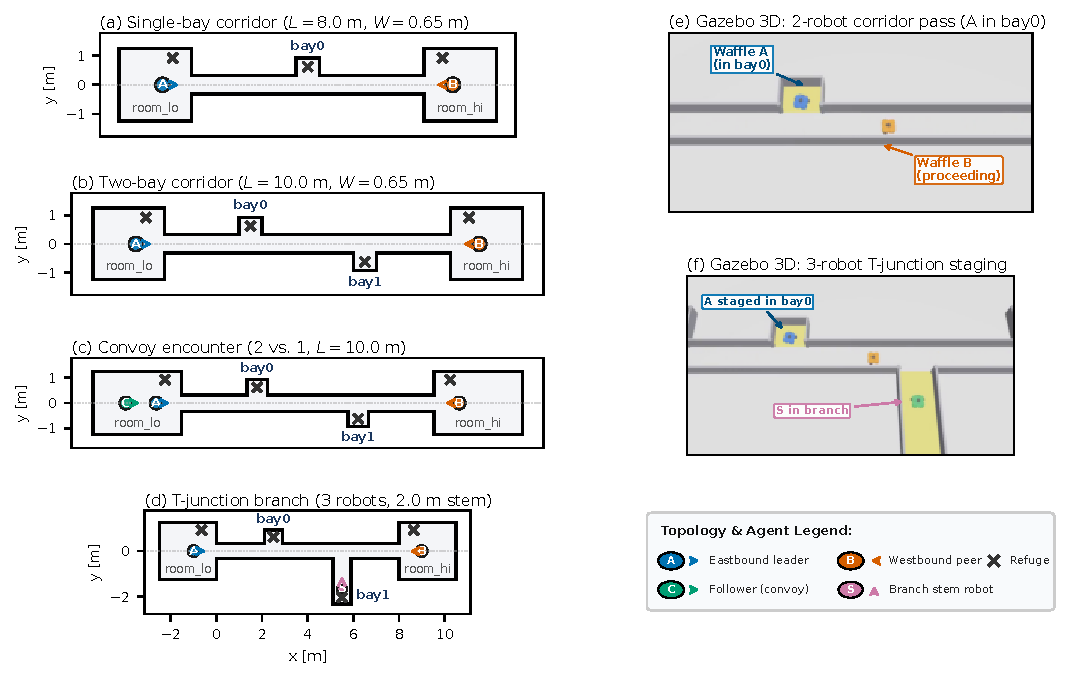
\includegraphics[width=1\textwidth]{Images/scenarios.pdf}
\caption{Benchmark scenario topologies and 3D validation environment. (a)--(d) Top-down 2D layouts (light gray: navigable space; $\times$: discrete refuge parking poses; colored discs/arrows: initial robot poses and travel directions). In (d), the turn-in variant is shown where robot~$S$ starts parked in the branch stem (\texttt{bay1}) and robot~$A$'s destination is \texttt{bay1}; in the exit variant, $A$ and $B$ traverse end-to-end while $S$ exits \texttt{bay1}. (e) Overhead capture from ROS~2 Jazzy / Gazebo Harmonic showing TurtleBot3 Waffle~$A$ parked in \texttt{bay0} while $B$ passes.}
\label{fig:scen}
\end{figure*}
Table~\ref{tab:design} details the complete experimental design across the four research questions (RQ1--RQ4), totaling 18 factorial 2D studies ($50{,}714$ simulated episodes) and 496 seed-paired ROS~2 / Gazebo Harmonic runs (460 main validation runs plus 36 hold-mode runs).

\begin{table*}[!t]\centering
\caption{Complete experimental design grouped by research question. Unless stated otherwise, parameters follow Table~\ref{tab:params}. $N$ counts simulated episodes (each hindsight reference evaluation executes two forced runs).}
\label{tab:design}
{\footnotesize\setlength{\tabcolsep}{3.4pt}
\begin{tabular}{@{}ll>{\raggedright\arraybackslash}p{0.35\textwidth}rlr@{}}\toprule
Layer / RQ & Study (Sec.) & Factorial Grid Factors & Seeds & Policies Evaluated & $N$ \\\midrule
\multirow{6}{*}{RQ1 (Sec.~\ref{sec:rq1})}
 & Single bay (\texttt{S1}) & Bay $x\in\{1,2,3,4,5,6,7\}$\,m & 60 & R, F, D, P, C, O, O$_w$ & 2,940 \\
 & Zone reservation & Bay $x\in\{1,\dots,7\}$\,m (separate 30-seed draw set) & 30 & S, F, D, C, forced A/B & 1,260 \\
 & Two bays (\texttt{S4}) & Bay 1 $\{2,3,4\}\times$ Bay 2 $\{6,7,8\}$\,m $\times$ side; B $U[0,10]$\,s & 20 & R, F, D, P, C, O, O$_w$ & 2,520 \\
 & Asymmetric robots (\texttt{S2}) & $u_B\in\{1,3\}\times$ load $\{0,1\}\times v_B\in\{0.26,0.13\}$\,m/s $\times$ bay $\{2,4,6\}$\,m & 30 & R, F, D, P, C, O, O$_w$ & 5,040 \\
 & Noisy bids (\texttt{S7}) & $\sigma\in\{0,0.1,0.25,0.5,1.0\}\times$ bay $x\in\{1,\dots,7\}$\,m & 30 & C, P, O & 3,150 \\
 & Learned classifier & Train: 800 two-bay pairs; Eval: 150 ID + 150 OOD & -- & L, F, D, C, O$_w$ & 1,600+1,500 \\\midrule
\multirow{3}{*}{RQ2 (Sec.~\ref{sec:rq2})}
 & Unpriced misreport (\texttt{S6}) & B bid scale $k\in\{1,1.5,2,4,10\}\times$ bay $x\in\{2,4,6\}$\,m & 60 & C, O & 1,080 \\
 & Clarke VCG (\texttt{S9}) & Deviator $\{\text{A, B, AB}\}\times 10$ scales $k\in[0.25,4]\times u_B\{1,3\}\times$ bay $\{2,4,6\}$ & 60 & V (+ none/naive eval) & 10,080 \\
 & Repeated fairness (\texttt{S10}) & 50 sequences $\times$ 20 encounters, bay $U[1,7]$\,m; $\lambda\in\{0,0.25,0.5,1,2\}$ & -- & forced A/B (offline) & 2,000 \\\midrule
\multirow{7}{*}{RQ3 (Sec.~\ref{sec:rq3})}
 & Comms sweep (\texttt{S3}) & Loss $\{0,10,30,50,70,90\}\%\times\tau\in\{0.05,0.25,0.5,1,2\}$\,s & 30 & F, D, P, C & 3,600 \\
 & Comms stress (\texttt{S8}) & $R_{\mathrm{det}}\{6,3,1.5\}$\,m $\times v\{0.26,0.5\}$\,m/s $\times$ loss $\{0,50,90\}\%\times\tau\{0.05,0.5,2\}$\,s & 20 & F, D, P, C & 4,320 \\
 & Extreme comms (\texttt{S8b}) & $R_{\mathrm{det}}\in\{1.5,6\}$\,m $\times$ loss $\{90,97,99\}\%\times\tau\in\{2,4,8\}$\,s; $v=0.5$\,m/s & 20 & F, D, P, C & 1,440 \\
 & Safeguard ablation (\texttt{S8c}) & \texttt{S8b} grid $\times$ \texttt{commit} $\{0,1\}\times$ \texttt{state\_guard} $\{0,1\}\times$ \texttt{bay\_check} $\{0,1\}$ & 20 & F, C & 5,760 \\
 & Asymmetric maps & 7 bay-knowledge splits $\times$ \texttt{share\_map} $\{0,1\}\times$ loss $\{0,50\}\%$; bays $3,7$\,m & 10 & F, D, C & 840 \\
 & Blocked bays & Physically obstructed bays $\in\{\emptyset,\text{bay0},\text{bay1},\text{both}\}\times$ loss $\{0,50\}\%$ & 10 & R, F, D, C & 320 \\
 & Explore \& hold & 4 map modes $\times R_{\mathrm{det}}\in\{6,3.5\}$\,m $\times$ loss $\{0,50\}\%$ (+ hold batch) & 30 & F, D, C & 1,440+360 \\\midrule
\multirow{3}{*}{RQ4 (Sec.~\ref{sec:rq4})}
 & Convoy 2 vs.\ 1 & B type (equal, loaded, $u_B=3$) $\times$ bays $\{2,4\}\times\{6,8\}\times$ delay $\{0,4,8\}\times$ loss & 3 & F, D, C, G, side ref. & 1,080 \\
 & T-junction (3 robots) & Delays $(A,B,S)\in\{0,4\}\times\{0,4,8\}\times\{0,6\}$\,s $\times 2$ S goals $\times$ loss $\{0,50\}\%$ & 2 & R, F, D, C & 384 \\
 & ROS~2 / Gazebo 3D & Seed-paired reduced grid across all studies + 36 hold/rerun runs & 6--10 & R, S, F, D, P, L, C, G, V, O & 460+36 \\\bottomrule
\end{tabular}}
\end{table*}

\subsection{Evaluation Metrics, Hindsight Reference, and Statistical Rigor}
Episodes run until all robots reach their goals or the time limit $T_{\max} = 180.0$\,s expires. Each episode records (1)~\emph{success} (all goals reached within 180\,s with zero collisions); (2)~\emph{deadlock} (180\,s reached without collision); (3)~\emph{collision} (SAT overlap of chassis footprints or entering within 0.50\,m of an obstacle); (4)~free-flow-subtracted \emph{delay} $D = \sum_i w_i(T_i - T_i^{\mathrm{free}})$, evaluated unweighted ($w_i = 1$) or urgency-weighted ($w_i = u_i$); (5)~\emph{reverse distance}; and (6)~\emph{first-yielder identity}. (Diagnostic \texttt{min\_clearance} logs axle distance minus $2R_{\mathrm{sw}} = 0.50$\,m, which can turn slightly negative before front bumper contact.)
Because raw delay $D$ conflates policy decision quality with encounter geometry (robots meeting far from any bay incur delay under \emph{any} policy), for every encounter $k$, both forced outcomes, i.e., \texttt{forced\_A} and \texttt{forced\_B}, are simulated, defining the hindsight \emph{best forced yielder} reference $\min(D_A^{(k)}, D_B^{(k)})$. Policy $\pi$'s paired \emph{excess delay} across $N$ encounters is given by
\begin{equation}
\Delta_\pi = \frac{1}{N}\sum_{k=1}^{N}\Bigl(D_\pi^{(k)} - \min\bigl(D_A^{(k)}, D_B^{(k)}\bigr)\Bigr).
\label{eq:excess}
\end{equation}
Here, $\Delta_\pi = 0$ indicates that $\pi$ selected the better yielder on every encounter. Because the reference optimizes only \emph{who} yields under immediate execution, policies that alter conflict timing (e.g., \texttt{hold\_for\_map}) can occasionally achieve $\Delta_\pi < 0$. For 2-vs.-1 convoys, an analogous \texttt{side\_oracle} takes the minimum delay of forcing the convoy vs.\ the lone robot to yield.
All reported statistics reflect the final codebase, apart from explicitly noted pre-fix failure counts that motivated protocol additions. Seed-matched encounters ensure identical start delays and wireless channel noise across all policies. Delays are averaged over successful episodes only, providing a conservative lower bound whenever a policy experiences deadlocks. Uncertainties ($\pm$) denote 95\% confidence intervals (paired per-encounter for $\Delta_\pi$), proportions carry Wilson 95\% intervals, and zero-collision counts report Wilson 95\% upper bounds.
\section{Results}\label{sec:results}
This section evaluates the benchmarked policies across RQ1--RQ4, progressing from decision-layer information and cost noise (Sec.~\ref{sec:rq1}) and strategic incentives (Sec.~\ref{sec:rq2}) to execution-layer channel and map resilience (Sec.~\ref{sec:rq3}) and multi-robot 3D Gazebo transfer (Sec.~\ref{sec:rq4}).

\subsection{Information, Geometry, Cost Noise, and Generalization (RQ1)}\label{sec:rq1}
The single-bay baseline (\texttt{S1}, with 7 bay positions $\times$ 60 seeds = 420 episodes per policy) first tests whether inter-robot communication is necessary. Without communication, the \texttt{reactive} baseline succeeded in $93.8\%$ [91.1--95.7\%] of encounters, deadlocking in the remaining 26 episodes when random patience timers failed to break symmetry before the $180$\,s time limit. Even when successful, \texttt{reactive} was slow and inefficient; it averaged $97.1\pm4.5$\,s of total delay against $26.8\pm0.6$\,s for the hindsight reference, a $3.6\times$ penalty. Because the 26 deadlocked episodes are excluded, this is a lower bound; charging both robots the full $180$\,s in every deadlocked episode bounds the mean at $113$\,s ($4.2\times$). Because the robots could not coordinate their intent, both backed up simultaneously in $39\%$ of episodes, driving an average of $5.7$\,m in reverse versus $0.64$\,m for the reference. By contrast, all four negotiating policies in \texttt{S1} (\texttt{fixed\_priority}, \texttt{rules\_default}, \texttt{rules\_proximity}, and \cb) completed $100\%$ of episodes (420/420) with zero collisions. Although \texttt{fixed\_priority} could in principle operate without radio if robot IDs were sensed visually, here it uses the broadcast protocol; thus, its gain over \texttt{reactive} reflects the combined benefit of a shared tie-breaking rule and explicit message passing. A stronger zero-communication baseline, randomized exponential backoff (\texttt{backoff}, patience drawn from $U[0, 6\cdot2^{k}]$\,s after $k$ earlier yields; study \texttt{S11b}), raises completion to $96.7\%$ but not efficiency ($92.3\pm6.3$\,s excess delay vs.\ $6.5\pm0.6$\,s for \texttt{fixed\_priority}). One-at-a-time sweeps of every rulebook threshold on the \texttt{S1}, \texttt{S2}, and \texttt{S4} grids (\texttt{S11a}) left excess delay unchanged except for the urgency threshold, which at $2.5$ raises \texttt{S2} weighted excess from $3.5$ to $15.7$\,s (\texttt{rules\_default}).

While any shared tie-breaking rule eliminates symmetric deadlocks, encounter efficiency depends strongly on how policies exploit corridor geometry. Figure~\ref{fig:rq1_geom} shows how excess delay $\Delta_\pi$ varies with pull-in bay position $x\in\{1,\dots,7\}$\,m for symmetric robots. Under \texttt{fixed\_priority} and \texttt{rules\_default} (which coincide when robots have equal urgency and load, because robot $A$ always enters at $t=0$ ahead of delayed robot $B$), excess delay averages $6.4\pm 0.6$\,s overall, spiking to $14.6$--$14.8$\,s when the bay sits near $A$'s entrance ($x=2$--$3$\,m), where $B$ is forced to reverse all the way back to \texttt{room\_hi} even when $A$ has just passed a nearby bay. Promoting geometric proximity ahead of corridor seniority (\texttt{rules\_proximity}) halves overall excess delay to $3.1\pm 0.5$\,s. Residual peaks remain at $x=3$\,m ($14.8$\,s) and $x=4$\,m ($7.1$\,s), where \texttt{rules\_proximity} makes exactly the same choices as \texttt{fixed\_priority}: $A$ has slightly passed the bay at conflict detection, yet reversing $A$ into it remains cheaper than reversing $B$ out of the aisle. This advantage is layout-specific: in the two-bay corridor (\texttt{S4}, 360 encounters), \texttt{rules\_proximity} incurs $5.6\pm 0.5$\,s of excess delay and picks the hindsight yielder in only $14\%$ of encounters, worse than both \texttt{fixed\_priority} ($1.1\pm 0.3$\,s) and \texttt{rules\_default} ($1.2\pm 0.3$\,s), because the nearest refuge is often not the cheaper one when a second bay is available.

\begin{figure}[!t]\centering
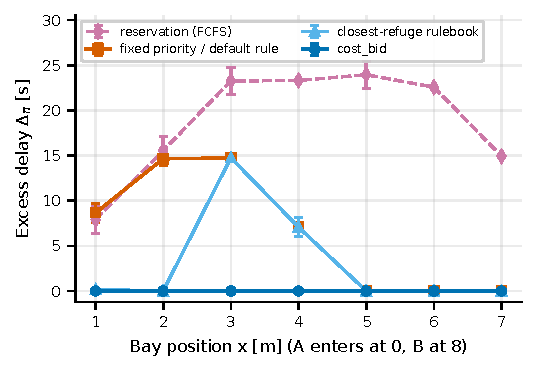
\includegraphics[width=\columnwidth]{Images/fig5_bay_geometry.pdf}
\caption{Mean excess delay $\Delta_\pi$~\eqref{eq:excess} versus pull-in bay coordinate $x$ in the single-bay corridor across negotiating policies (\texttt{S1}) and first-come corridor mutex locking (\texttt{reservation}). Error bars show 95\% CIs.}
\label{fig:rq1_geom}
\end{figure}

By comparison, coarse corridor-level locking ignores intermediate pull-in bays altogether. First-come corridor reservation (\texttt{reservation}, evaluated over 210 encounters across $x\in\{1,\dots,7\}$\,m in Fig.~\ref{fig:rq1_geom}) completed $100\%$ of episodes without collision, but incurred $18.8\pm 0.9$\,s of excess delay. This delay is nearly triple that of \texttt{fixed\_priority} ($6.5\pm 0.9$\,s on the same draws), and \texttt{reservation} never outperformed the best forced yielder ($0/210$ encounters). Because Robot~$B$ starts directly on Robot~$A$'s exit path, waiting outside the corridor forces $B$ to turn and park off-lane inside \texttt{room\_hi} (adding $\sim 17$\,s of maneuver overhead) while waiting for $A$ to traverse the entire aisle rather than using an intermediate bay. Facility layouts where staging areas already sit clear of the exit lane would penalize reservation less severely. At the other extreme, noise-free \cb\ selected the exact same yielder as the hindsight reference in $100\%$ of single-bay (\texttt{S1}, 420 encounters) and two-bay (\texttt{S4}, 360 encounters) episodes ($\Delta_\pi = 0.0$\,s). Because \cb\ uses the true speed limits and refuge coordinates of the deterministic simulator, this exact match primarily validates the cost model. Omitting acceleration and turning transients produces a mean absolute prediction error of $1.9$\,s per robot (up to $4.0$\,s across 780 episodes), yet in symmetric corridors that error is never large enough to flip which robot should yield.

\begin{figure}[!t]\centering
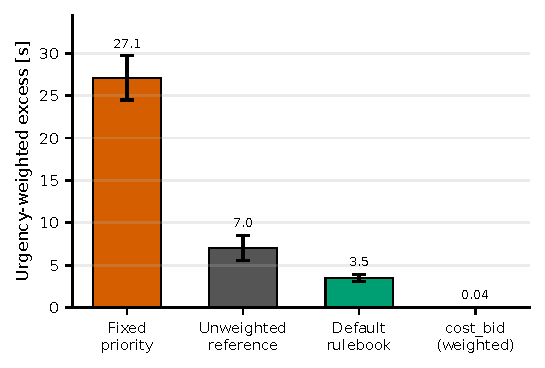
\includegraphics[width=\columnwidth]{Images/fig6_asymmetry.pdf}
\caption{Urgency-weighted excess delay across heterogeneous robot urgency, payload, and speed regimes (\texttt{S2}, $N=5{,}040$). Error bars show 95\% CIs.}
\label{fig:rq1_asym}
\end{figure}

Moving from identical robots to mixed fleets highlights the trade-off between simple priority rules and estimating actual maneuver delays. In study \texttt{S2} (5,040 episodes, Fig.~\ref{fig:rq1_asym}), where robots differ in urgency ($u_B\in\{1,3\}$), payload status, and top speed ($v_B\in\{0.26,0.13\}$\,m/s), static ID priority (\texttt{fixed\_priority}) performs poorly. It incurs $27.1\pm 2.6$\,s of urgency-weighted excess delay because Robot~$B$ is forced into long reverse maneuvers even when carrying an urgent load or moving at half speed. Adding simple urgency and payload rules (\texttt{rules\_default}) reduces this weighted excess delay nearly eightfold to $3.5\pm 0.4$\,s. Crucially, the hindsight reference that minimizes \emph{unweighted} total delay (\texttt{oracle}) still incurs $7.0\pm 1.5$\,s of urgency-weighted excess delay. Thus, optimizing the wrong fleet objective wastes twice as much weighted time as replacing a kinematic planner with a heuristic rulebook. By contrast, urgency-weighted \cb\ reduces weighted excess delay to just $0.04\pm 0.02$\,s and picks the same yielder as the weighted reference (\texttt{oracle\_w}) in $98\%$ of encounters (704/720). The 16 remaining encounters are all close near-ties where unmodeled acceleration and turning transients slightly shift the outcome, having a median predicted bid difference of only $0.6$\,s (maximum $2.2$\,s) compared with $12.4$\,s across the 704 agreed encounters.

In real-world deployments, however, robots cannot predict their maneuver delays exactly due to floor friction, battery sag, and localization jitter. To test how sensitive \cb\ is to estimation errors, study \texttt{S7} (single-bay corridor, Fig.~\ref{fig:rq1_noise}) multiplies each robot's predicted bid by log-normal noise $e^{\sigma\epsilon}$. As the noise level $\sigma$ increases, the excess delay of \cb\ rises from $0.0$\,s ($\sigma=0$) to $0.15\pm 0.15$\,s ($\sigma=0.1$), $1.5\pm 0.6$\,s ($\sigma=0.25$), $3.3\pm 0.8$\,s ($\sigma=0.5$), and $4.5\pm 0.9$\,s ($\sigma=1.0$). Once bid noise reaches $\sigma=0.5$ (where bids typically vary by a factor of $e^{0.5}\approx 1.65\times$), noisy \cb\ offers no statistical advantage over the simple closest-refuge rulebook (\texttt{rules\_proximity}, $3.2\pm 0.8$\,s on the same draws), and remains clearly better only when $\sigma\le 0.25$; at $\sigma=1.0$ the rulebook is ahead by a paired $1.3\pm 1.2$\,s. Because \texttt{rules\_proximity} itself trails fixed priority in the two-bay layout, this crossover should not be generalized beyond single-bay corridors. Note that study \texttt{S7} adds random noise to the final bid value, whereas systematic model errors (such as a miscalibrated reverse speed $v_{\mathrm{rev}}$) remain an open direction for future testing.

\begin{figure}[!t]\centering
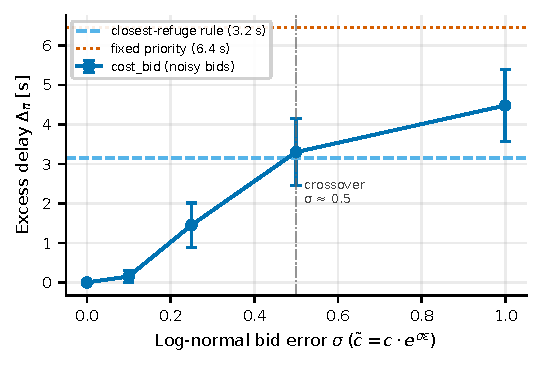
\includegraphics[width=\columnwidth]{Images/fig7_bid_noise.pdf}
\caption{Sensitivity of \cb\ excess delay $\Delta_\pi$ to multiplicative log-normal bid estimation error $\sigma$ (\texttt{S7}, $N=3{,}150$), reaching parity with noise-free \texttt{rules\_proximity} at $\sigma\approx 0.5$. Error bars show 95\% CIs.}
\label{fig:rq1_noise}
\end{figure}

Instead of using a formula to estimate maneuver delays, a policy can learn which robot should yield directly from past encounters. Figure~\ref{fig:rq1_bandit} shows that on the two-bay corridor layout where it was trained, the tabular full-information outcome classifier (\texttt{learned}) matches the performance of \texttt{rules\_default} on held-out test episodes ($+2.6$\,s vs.\ $+2.5$\,s weighted excess delay; a table trained on only $200$ encounters already reaches $+2.8$\,s) without relying on an explicit motion model. However, when tested on an unseen single-bay corridor with randomized bay positions, its excess delay jumps to $+13.1$\,s. This performance is worse than both \texttt{fixed\_priority} ($+12.3$\,s) and \texttt{rules\_default} ($+6.3$\,s), with $15\%$ of encounters falling into state bins never seen during training. Because the classifier only looks at coarse distance bins to the nearest refuge behind each robot and ignores where the oncoming robot can stop relative to each bay, the lookup table memorizes layout-specific patterns rather than general corridor physics.

\begin{figure}[!t]\centering
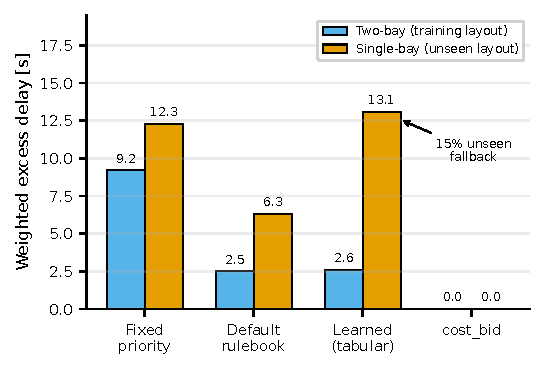
\includegraphics[width=\columnwidth]{Images/fig8_bandit_generalization.pdf}
\caption{Tabular outcome classifier (\texttt{learned}) weighted excess delay on its training two-bay layout versus an unseen single-bay layout ($150$ evaluation episodes per layout).}
\label{fig:rq1_bandit}
\end{figure}



\subsection{Strategic Incentives and Repeated-Encounter Fairness (RQ2)}\label{sec:rq2}
The strong performance of \cb\ in Section~\ref{sec:rq1} assumes that every robot reports its delay cost honestly. In a multi-vendor facility, however, a self-interested robot can exaggerate its predicted delay to avoid yielding. In study \texttt{S6} (1,080 episodes), where the lower bid yields without any payment, if Robot~$B$ multiplies its reported bid by $k\ge 2\times$, it forces Robot~$A$ to yield in $100\%$ of encounters. As a result, $B$'s own mean delay drops from $9.1\pm 1.4$\,s to $8.1\pm 1.2$\,s, while the combined fleet delay increases by $+4.9$\,s ($+20\%$). Similarly, in the unpriced baseline of study \texttt{S9} (dashed orange curve in Fig.~\ref{fig:rq2_misreport}), Robot~$A$ gains up to $+4.74\pm 0.99$\,s of individual utility by inflating its bid by $k=4\times$. Simply making the proceeding robot pay the yielding robot's reported bid does not encourage honesty either. Instead, this naive side-payment reverses the incentive to lie (dotted purple curve in Fig.~\ref{fig:rq2_misreport}), allowing Robot~$A$ to gain $+7.54\pm 1.76$\,s by \emph{under-reporting} its cost at $k=0.25\times$ to manipulate the payment terms, while Robot~$B$ gains $+0.68$\,s at $k=0.75\times$.

\begin{figure}[!t]\centering
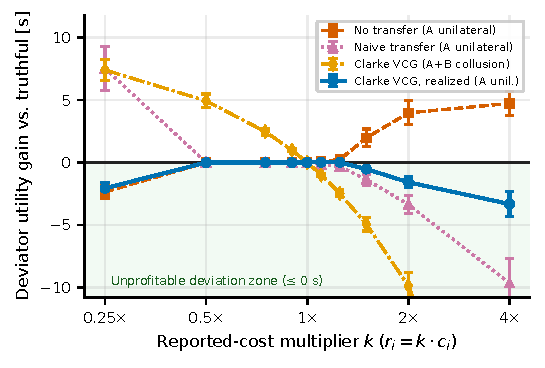
\includegraphics[width=\columnwidth]{Images/fig9_strategic_misreport.pdf}
\caption{Deviator single-encounter utility gain (seconds of urgency-weighted delay plus transfer) relative to truthful reporting ($k=1\times$) across $N=10{,}080$ episodes in \texttt{S9}; values $\le 0$\,s (shaded green) indicate unprofitable deviations. Error bars show 95\% CIs.}
\label{fig:rq2_misreport}
\end{figure}

To make honest reporting the best choice for each individual robot, study \texttt{S9} evaluates the Clarke-pivot mechanism (Eq.~\eqref{eq:clarke}) across 6 bay and urgency settings, 27 unilateral and joint misreport conditions (deviator $\in\{A, B, AB\}\times$ nine non-truthful scales $k\in\{0.25, 0.5, 0.75, 0.9, 1.1, 1.25, 1.5, 2, 4\}$) plus the truthful baseline ($k=1$), and 60 seeds (10,080 episodes total, all completing without collision). Under the planner's predicted costs, \emph{no} single-robot misreport ($0/108$ deviator conditions across Robots~$A$ and~$B$) improves the lying robot's utility ($0.00$\,s maximum gain), confirming that truthful bidding is an exact dominant strategy. When utility is measured using the \emph{actual} simulated travel times (which differ slightly from the planner's predictions due to acceleration and turning transients), lying unilaterally costs Robot~$A$ up to $-3.3\pm 1.0$\,s of utility at extreme scaling factors (solid blue curve in Fig.~\ref{fig:rq2_misreport}) and Robot~$B$ up to $-4.9\pm 1.2$\,s (at $k=0.25\times$). Across the entire test grid, the largest realized gain from misreporting is just $+0.02\pm 0.02$\,s (at $k=1.1\times$), which is statistically indistinguishable from zero. Because both robots' types are computed from shared kinematic snapshots, this result is an implementation check of the mechanism rather than evidence of robustness to private information. With private urgency and independent per-outcome misreports (\texttt{S9b}, 10,080 deviating episodes), no deviation improved the deviator's predicted utility; realized gains above $0.01$\,s occurred in 89 episodes ($0.9\%$), all caused by execution departing from the predicted plan, and the mean realized gain was negative in every arm.


\begin{figure}[!t]\centering
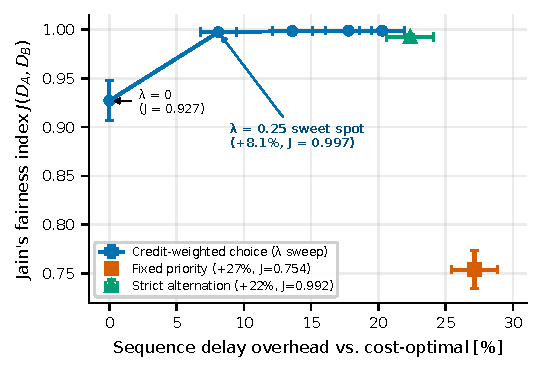
\includegraphics[width=\columnwidth]{Images/fig10_fairness_pareto.pdf}
\caption{Repeated-encounter Pareto frontier (\texttt{S10}, 50 sequences of 20 encounters) trading sequence delay overhead against cumulative Jain fairness $J(D_A^{\mathrm{cum}}, D_B^{\mathrm{cum}})$ as credit weight $\lambda$~\eqref{eq:karma} varies from $0$ to $2.0$. Error bars show 95\% CIs.}
\label{fig:rq2_fairness}
\end{figure}

At the same time, study \texttt{S9} highlights three practical limitations that fleet engineers must consider before deploying a Clarke-pivot (VCG) mechanism.
\begin{enumerate}
\item \emph{Chronic budget surplus.} In line with the Green--Laffont impossibility theorem~\cite{green1977characterization}, payments cannot simply be transferred from one encountering robot to the other and must instead be paid into an external fleet bank. This bank collects an average surplus of $9.3\pm 1.6$\,s of delay credit per encounter when $u_B=1$ ($44\%$ of the planner-predicted total delay cost, or $37\%$ of the realized urgency-weighted delay) and $10.5\pm 1.5$\,s when $u_B=3$ ($29\%$ predicted, $24\%$ realized), meaning the facility must periodically redistribute accumulated credits outside the real-time negotiation loop.
\item \emph{Vulnerability to joint collusion.} If Robot~$A$ and Robot~$B$ both scale their reported costs down by the same factor $k<1$, the chosen yielder $o^\ast$ stays the same while both robots' payments shrink by a factor of $k$. Under joint $0.5\times$ bid shading, their combined utility improves by $+4.94\pm 0.55$\,s (and by $+7.42$\,s at $0.25\times$, shown by the dash-dotted gold curve in Fig.~\ref{fig:rq2_misreport}).
\item \emph{Mandatory participation and non-bid cheating.} Compared with a static \texttt{fixed\_priority} policy where Robot~$A$ always has the right-of-way and pays nothing, Robot~$A$ is worse off under the Clarke mechanism in $100\%$ of encounters (losing an average of $9.3$\,s per encounter at $u_B=1$ and $10.5$\,s at $u_B=3$). Thus, high-priority robots will only participate if required by the facility operator. Furthermore, VCG only guarantees honesty for the reported cost numbers $b_i(o)$ and assumes robots follow the protocol honestly in other respects. A robot could still cheat outside the bidding math by omitting a known pull-in bay from its \texttt{BID} message to shrink the feasible refuge set $\mathcal{F}$, or by spoofing a lower robot ID to win \texttt{commit} tie-breakers.
\end{enumerate}

While multi-vendor fleets need payment mechanisms to ensure truthful bidding, single-owner cooperative fleets already share a common goal, yet can still suffer from unfair delays across repeated encounters if tie-breaking rules always favor the same robot. Across 50 sequences of 20 random single-bay encounters (study \texttt{S10}, Fig.~\ref{fig:rq2_fairness}), \texttt{fixed\_priority} forces Robot~$B$ to yield every time. This one-sided rule drops cumulative Jain fairness to $J=0.754$ while increasing total fleet delay by $+27.1\%$ compared with cost-optimal selection. Notably, pure cost-optimal selection ($\lambda=0$) already achieves high fairness ($J=0.927$) because random bay locations and start delays naturally vary which robot is closer to a refuge. Forcing the robots to strictly take turns yielding (\texttt{alternate}) raises fairness to $J=0.992$, but adds $+22.3\%$ of extra delay because it ignores corridor geometry. Choosing the fairness weight in Eq.~\eqref{eq:karma} on these 50 sequences (smallest-overhead $\lambda$ with $J\ge0.99$, giving $\lambda=0.1$) and evaluating it closed-loop on 100 fresh sequences (\texttt{S10b}) yields $J=0.992$ at $+3.8\pm0.6\%$ extra delay; with log-normal error on the delay estimates the overhead grows to $+7.1\%$ ($\sigma=0.25$) and $+11.5\%$ ($\sigma=0.5$) at unchanged $J\approx0.99$. The absolute-gap variant $\lambda\,|(D_A+d_A(o))-(D_B+d_B(o))|$ selects $\lambda=0.25$ and gives $J=0.994$ at $+3.0\%$. With a small $\lambda$, the rule follows the cost-optimal decision on clear-cut encounters and only flips close near-ties in favor of whichever robot has accumulated more past delay. This cumulative-delay ledger is kept strictly separate from the Clarke VCG payments in study \texttt{S9}, because carrying VCG credits over as a spending budget across multiple encounters would break the single-encounter truthfulness guarantee.


\subsection{Channel Impairment, Safeguard Ablation, and Map Uncertainty (RQ3)}\label{sec:rq3}
Having evaluated the decision policies under ideal communication, the next experiments test how the distributed execution protocol holds up when wireless links degrade. Across both moderate and heavy channel impairment in study \texttt{S3} (packet loss from $0\%$ to $90\%$ and latency from $0.05$\,s to $2.0$\,s over 3,600 episodes) and study \texttt{S8} (detection range $R_{\mathrm{det}}\in\{6,3,1.5\}$\,m, top speed $v_{\max}\in\{0.26,0.5\}$\,m/s, packet loss up to $90\%$, and latency up to $2.0$\,s over 4,320 episodes), every negotiating policy (\texttt{fixed\_priority}, \texttt{rules\_default}, \texttt{rules\_proximity}, and \cb) completed $\ge 99.3\%$ of encounters pooled over each study's grid (the hardest individual cells, at $90\%$ loss, still reached $\ge 90\%$) with \emph{zero collisions} (Fig.~\ref{fig:rq3_comms}). Mean delay stayed nearly flat (varying by only $1$--$2$\,s) up to $50\%$ packet loss because resending \texttt{BID} messages every $0.3$\,s reliably delivers both snapshots well before the robots physically meet. Delay rises gradually only above $70\%$ packet loss, where the $3.0$\,s negotiation timeout occasionally expires and triggers a reactive backoff fallback. Completion therefore overstates how often negotiation itself succeeds: at the most extreme loss levels of \texttt{S8b}/\texttt{S8c}, $62.8\%$ of episodes recorded no negotiated decision and were resolved by the reactive fallback. On fresh seeds with correlated loss (study \texttt{S8d}, 2,560 episodes; Gilbert--Elliott bursts of mean length 5--100 messages and total blackouts of 10--40\,s), no collision occurred and $\ge 99.4\%$ of encounters completed, but only $71.9\%$ of bursty-loss and $92.5\%$ of blackout episodes reached a negotiated decision.

\begin{figure}[!t]\centering
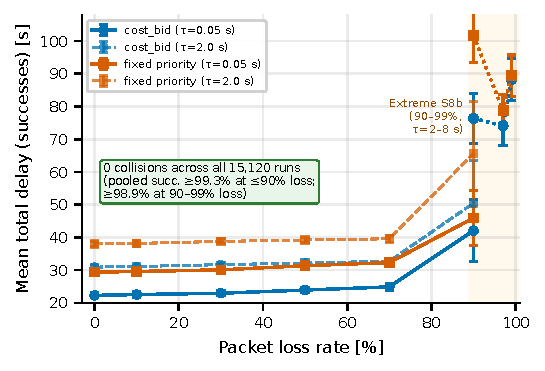
\includegraphics[width=\columnwidth]{Images/fig11_comms_resilience.pdf}
\caption{Mean total delay over successful episodes across packet loss $0$--$99\%$ and base latency $\tau\in[0.05, 8.0]$\,s (\texttt{S3} at $0.26$\,m/s and extreme \texttt{S8b} shaded right at $0.50$\,m/s); zero collisions occurred across all 15,120 communication-sweep and ablation episodes. Error bars show 95\% CIs.}
\label{fig:rq3_comms}
\end{figure}

Under extreme channel impairment in study \texttt{S8b} ($90\%$ to $99\%$ packet loss, $2$\,s to $8$\,s latency, and $v_{\max}=0.5$\,m/s across 1,440 episodes), an early version of the agent experienced 6 collisions when both robots yielded on mismatched snapshots and pulled back out into the corridor at the same time. After tightening the lane-clearance and bay-exit checks in the final protocol, all four negotiating policies recorded \emph{zero collisions} across all 1,440 episodes in \texttt{S8b}, achieving $98.9\%$ to $99.2\%$ completion. (Note that studies \texttt{S8b} and \texttt{S8c} used a higher top speed of $0.5$\,m/s in 2D to stress-test fast closing speeds, whereas the extreme-communication runs in Gazebo used the standard TurtleBot3 Waffle speed of $0.26$\,m/s.)

To test which protocol safeguard actually prevents collisions, study \texttt{S8c} (Table~\ref{tab:abl}, 5,760 episodes) turns \texttt{commit}, \texttt{state\_guard}, and \texttt{bay\_check} on and off in all $2^3$ combinations under the extreme packet-loss and latency settings of study \texttt{S8b}. Surprisingly, \emph{zero collisions occurred in every single test condition}, even when all three safeguards were turned off ($95\%$ upper bound of $1.06\%$ per 360-episode condition). Two factors explain why disabling the radio safeguards did not cause collisions. First, at a $5$\,Hz broadcast rate and $90\%$ to $99\%$ packet loss, the chance that a robot has no fresh ($<1$\,s) peer \texttt{STATE} message is $0.90^5=59\%$ to $0.99^5=95\%$, and any messages that do arrive are already $2$\,s to $8$\,s old. Physical collision avoidance under extreme loss therefore comes from local Lidar stopping margins and randomized $U[6,12]$\,s bay-exit wait timers rather than radio-based state guards. Second, \texttt{bay\_check} never triggered even once (all 8 conditions with \texttt{bay\_check} enabled produced the exact same episode outcomes as those with it disabled). Meanwhile, turning on \texttt{commit} added $3.1$\,s to $3.8$\,s of mean delay and actually \emph{increased} how often both robots started yielding at the same time (from $15.3\%$--$16.4\%$ to $21.9\%$--$23.6\%$ under \texttt{fixed\_priority}), because waiting for a dropped confirmation packet pushes robots past the $3.0$\,s negotiation timeout into reactive backoff. Small differences in deadlock counts across conditions (1 to 7 out of 360 episodes) fall within random sampling noise. Note that these temporary mutual yields ($14.2\%$ to $23.6\%$ of runs) have no theoretical guarantee of resolving within a fixed time, and the recorded deadlocks are simply episodes where mutual backoff lasted past the $180$\,s time limit.

\begin{table}[!t]\centering
\caption{Factorial safeguard ablation (\texttt{S8c}) under 90--99\% packet loss and 2--8\,s latency ($v_{\max}=0.5$\,m/s; 360 episodes per row; \texttt{bay\_check} had zero triggers and identical metrics, so its 8 duplicate rows are condensed). Collisions were 0 in every arm (95\% upper bound 1.06\%).}
\label{tab:abl}
{\footnotesize\setlength{\tabcolsep}{3.4pt}
\begin{tabular}{@{}lccrrrr@{}}\toprule
Policy & \texttt{commit} & \texttt{state} & Succ.\ [\%] & Deadl. & Delay [s] & Dual [\%] \\\midrule
\multirow{4}{*}{\texttt{fixed\_pr.}}
 & \checkmark & \checkmark & 99.2 & 3 & $89.8\pm3.9$ & 21.9 \\
 & \checkmark & --         & 99.2 & 3 & $90.0\pm4.0$ & 23.6 \\
 & --         & \checkmark & 98.1 & 7 & $86.0\pm3.6$ & 15.3 \\
 & --         & --         & 98.6 & 5 & $86.8\pm3.7$ & 16.4 \\\midrule
\multirow{4}{*}{\cb}
 & \checkmark & \checkmark & 98.9 & 4 & $79.6\pm3.9$ & 17.8 \\
 & \checkmark & --         & 99.2 & 3 & $79.9\pm3.9$ & 18.6 \\
 & --         & \checkmark & 99.4 & 2 & $76.4\pm3.7$ & 14.2 \\
 & --         & --         & 99.7 & 1 & $76.8\pm3.7$ & 14.7 \\\bottomrule
\end{tabular}}\\[2pt]
{\footnotesize \texttt{state}: \texttt{state\_guard}. Dual: \% of episodes where both robots entered \texttt{YIELD} before one aborted/exited.}
\end{table}

Beyond packet loss, decentralized robots may also start with incomplete or outdated maps of where pull-in bays are located. When two robots know different subsets of the bays in the two-bay corridor (840 episodes, 10 seeds per condition), no collisions or deadlocks occur because \texttt{commit} resolves any conflicting decisions in favor of the lower-ID robot (Robot~$A$). Extra delay occurs only when Robot~$A$ has the less complete map. If Robot~$A$ only knows about \texttt{bay0} ($x=3$\,m), \cb\ incurs $+9.1$\,s of extra delay and \texttt{fixed\_priority} and \texttt{rules\_default} incur $+29.6$\,s (at $0\%$ loss) because Robot~$B$ is sent all the way back to \texttt{room\_hi}. If Robot~$A$ knows neither bay, all policies incur $+30.9$\,s to $+31.1$\,s of extra delay. Simply attaching each robot's list of known bay IDs to every outgoing \texttt{BID} message (\texttt{share\_map}) removes $100\%$ of this extra delay ($+0.0$\,s) whenever at least one robot knows a bay, even at $50\%$ packet loss. Conversely, when a bay listed on the map is physically blocked by an unmapped obstacle such as a pallet (320 episodes), a naive Lidar occupancy check (\texttt{bay\_check}) deadlocked in $10/10$ runs because the yielding robot mistook the static obstacle for a peer robot already parked in the bay. Cross-checking the Lidar return against fresh peer \texttt{STATE} positions (\texttt{refuge\_blocked}) allowed the robot to recognize the bay as permanently blocked and broadcast it to its peer, restoring $10/10$ completion with zero collisions for every negotiating policy (adding $+46$\,s of delay when the useful bay, \texttt{bay1}, is blocked, because the blockage is only discovered once the robot reaches the bay); the non-negotiating \texttt{reactive} baseline still deadlocked in $2/10$ (\texttt{bay1} blocked) and $3/10$ (both blocked) runs.

When robots instead discover pull-in bays as they drive in \texttt{explore} mode (1,440 base episodes plus 360 hold-mode episodes in 2D, Fig.~\ref{fig:rq3_maps}), they start knowing only the end rooms and add each bay to their map once it comes within the $3.5$\,m Lidar range. At the default radio conflict-detection range of $R_{\mathrm{det}}=6.0$\,m, waiting to share discovered bays until the robots physically detect each other on Lidar (\texttt{share\_on\_detect}) fails completely. Because the robots freeze their snapshots and make a yield decision at $6.0$\,m apart, well before their $3.5$\,m Lidar ranges ever overlap ($0/30$ maps shared in time), \texttt{share\_on\_detect} suffers the exact same delay penalty as never sharing maps at all ($+29.2$\,s for \texttt{fixed\_priority} and the rulebooks, and $+8.8$\,s for \cb). In the 2D simulator, two workarounds recover full-map refuge choices ($-0.5$\,s to $+0.1$\,s extra delay compared with knowing the full map upfront). One option is shortening the radio conflict range $R_{\mathrm{det}}$ to $3.5$\,m to match the Lidar range, and the other is enabling \texttt{hold\_for\_map}, which keeps the robots driving forward undecided for $4.9$\,s to $5.5$\,s until they detect each other on Lidar and exchange maps. Even so, simply including known bays in every \texttt{BID} message (\texttt{share\_map}) achieves $+0.0$\,s extra delay right away at $6.0$\,m without holding up the decision.

\begin{figure}[!t]\centering
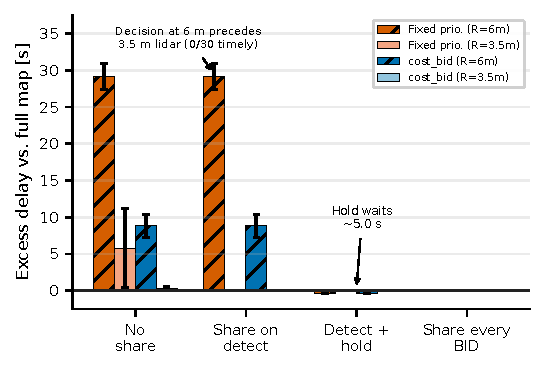
\includegraphics[width=\columnwidth]{Images/fig12_map_discovery.pdf}
\caption{Two-bay excess delay relative to full map knowledge in 2D \texttt{explore} mode ($0\%$ loss), showing why \texttt{share\_on\_detect} fails when radio negotiation ($R_{\mathrm{det}}=6$\,m) precedes $3.5$\,m Lidar range. Error bars show 95\% CIs.}
\label{fig:rq3_maps}
\end{figure}

\subsection{Three-Robot Topologies and Sim-to-3D Gazebo Transfer (RQ4)}\label{sec:rq4}
Pairwise negotiation rules must also handle multi-robot encounters where a third robot can physically block a yielding robot. In the 2-vs.-1 convoy study (1,080 episodes where follower~$C$ trails leader~$A$ against oncoming Robot~$B$, with 72 runs per policy and $B$-configuration pooled across $0\%$ and $50\%$ packet loss, Fig.~\ref{fig:rq4_convoy}), standard pairwise yielding traps a reversing leader against its own follower. Adding the local \texttt{make\_room} rule, which directs a blocking follower to back into an upstream refuge, eliminates all convoy deadlocks and achieves $72/72$ completion across every policy. The default rulebook, however, performs worst among the negotiating policies in every convoy regime ($40.0$\,s with equal robots, $100.1$\,s with loaded~$B$, and $133.6$\,s weighted with urgent~$B$, versus $33.7$, $33.7$, and $90.3$\,s for \texttt{fixed\_priority}), because its payload and urgency rules always make the two-robot convoy yield to a loaded or urgent lone robot, even when reversing the whole convoy is the costlier choice. When all robots have equal urgency ($u_A=u_C=u_B=1$), pairwise \cb\ only estimates the delay for leader~$A$ to reverse and ignores follower~$C$, resulting in an average delay of $55.6$\,s. Accounting for the whole convoy via \gb~\eqref{eq:groupbid} cuts mean delay to $34.4$\,s, coming within $+0.7\pm 1.4$\,s (paired difference) of both \texttt{fixed\_priority} and the hindsight side-level reference \texttt{side\_oracle} ($33.7$\,s). When the lone oncoming Robot~$B$ is urgent ($u_B=3$), however, \gb\ ($104.7\pm 6.7$\,s weighted delay) beats pairwise \cb\ ($117.1\pm 6.3$\,s, a paired improvement of $12.4\pm 5.8$\,s) but falls behind \texttt{fixed\_priority} ($90.3\pm 4.2$\,s, a paired gap of $+14.4\pm 8.0$\,s) and \texttt{side\_oracle} ($85.7\pm 3.1$\,s, a paired gap of $+19.0\pm 6.9$\,s). Because Eq.~\eqref{eq:groupbid} simply adds the individual yield delays of $A$ and $C$ together instead of modeling the extra time leader~$A$ must wait while follower~$C$ reverses out of the way first, \gb\ underestimates how long the convoy takes to yield and occasionally makes the convoy yield when backing lone Robot~$B$ into a nearby bay would actually be faster.

\begin{figure}[!t]\centering
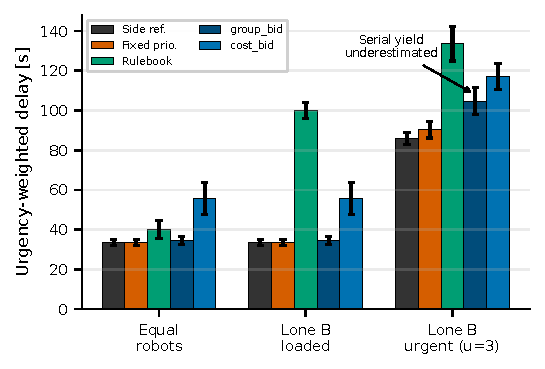
\includegraphics[width=\columnwidth]{Images/fig13_convoy_delay.pdf}
\caption{Convoy 2-vs.-1 urgency-weighted delay ($N=1{,}080$) across equal, loaded-$B$, and urgent-$B$ ($u_B=3$) regimes with follower \texttt{make\_room}. Error bars show 95\% CIs.}
\label{fig:rq4_convoy}
\end{figure}

\begin{figure}[!t]\centering
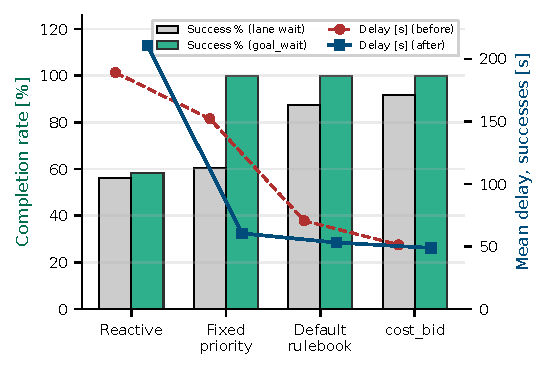
\includegraphics[width=\columnwidth]{Images/fig14_tjunction_goalwait.pdf}
\caption{Three-robot T-junction turn-in completion rate (bars, left axis) and successful-episode delay (lines, right axis) at $0\%$ loss ($n=48$ per policy) before versus after adding upstream bay waiting (\texttt{goal\_wait}).}
\label{fig:rq4_tjunction}
\end{figure}

A similar three-robot bottleneck occurs at branch intersections. In the T-junction turn-in study (384 episodes where Robot~$A$ is heading into branch \texttt{bay1} while Robot~$S$ is still inside \texttt{bay1} and Robot~$B$ is driving down the main corridor, with 48 runs per policy and packet-loss level, Fig.~\ref{fig:rq4_tjunction}), letting Robot~$A$ wait in the main corridor while \texttt{bay1} was occupied caused \texttt{fixed\_priority} to deadlock in $19/48$ runs ($60.4\%$ completion) at $0\%$ packet loss. Adding the \texttt{goal\_wait} rule, which directs Robot~$A$ to pull into the upstream refuge \texttt{bay0} until its target branch \texttt{bay1} clears, raised completion to $48/48$ ($100\%$) at both $0\%$ and $50\%$ packet loss for \texttt{fixed\_priority}, \texttt{rules\_default}, and \cb\ (compared with only $28/48$ for \texttt{reactive}, where all failures were deadlocks). With \texttt{goal\_wait} enabled at $0\%$ packet loss, mean total delay dropped from $60.5\pm 4.7$\,s under \texttt{fixed\_priority} to $53.1\pm 5.0$\,s under \texttt{rules\_default} and $48.9\pm 4.0$\,s under \cb\ (a paired improvement of $-4.3\pm 2.8$\,s over the rulebook).

Finally, to test whether the 2D results hold up under 3D rigid-body physics, planar LaserScan wall-filtering, and asynchronous ROS~2 message timing\label{sec:gz}, transfer was evaluated across 460 main validation runs in Gazebo Harmonic covering every study above (6 to 10 seeds per condition, taking $\sim 5$\,min of wall-clock time per episode including launch and reset) plus an additional 36-run explore-hold batch. Every Gazebo run was paired with a 2D simulation run using the exact same random seed (Table~\ref{tab:gz} and Fig.~\ref{fig:rq4_gz_scatter}). Within the 460-run main batch, 122 runs were executed on the code commit right before the explore and blocked-bay world features were added, and 338 were executed on the final commit (which did not change any behavior on default configurations), while all 36 hold-batch runs were executed on the final merged commit.

\begin{table}[!t]\centering
\caption{Seed-paired ROS~2 Jazzy / Gazebo Harmonic transfer summary (460 main validation runs + 36 hold/rerun batch runs).}
\label{tab:gz}
{\footnotesize\setlength{\tabcolsep}{3.0pt}
\begin{tabular}{@{}lrrrrr@{}}\toprule
Scenario / Study Group & Runs & Succ. & Coll. & Same & $\Delta D$ [s] \\\midrule
Single bay, negotiating (\texttt{S1}, S, L) & 70 & 70 & 0 & 70 & $-0.4$ \\
Single bay, \texttt{reactive}               & 10 &  9 & 1 &  5 & $-1.5$ \\
Forced yielders, S1 + S2 (O)             & 44 & 44 & 0 & 44 & $-0.5$ \\
Asymmetric urgency / speed (\texttt{S2}, neg.)    & 36 & 36 & 0 & 36 & $-0.6$ \\
Two bays (\texttt{S4})                      & 30 & 30 & 0 & 30 & $-0.2$ \\
Noisy bids ($\sigma=0.5, 1.0$; \texttt{S7}) & 12 & 12 & 0 &  7 & $+2.2$ \\
Clarke VCG misreports (\texttt{S9})         & 18 & 18 & 0 & 18 & $-0.3$ \\
50\% loss, $0.5$\,s latency (\texttt{S3})   & 18 & 18 & 0 & 18 & $-0.8$ \\
90\% loss, $2.0$\,s latency (\texttt{S8b/c})& 24 & 24 & 0 & 18 & $+4.8$ \\
Convoy 2 vs.\ 1 (\texttt{make\_room})       & 36 & 36 & 0 & 36 & $-0.6$ \\
T-junction (18 exit + 18 turn-in)           & 36 & 36 & 0 & 35 & $-16.8$ \\
Asymmetric static maps                      & 24 & 24 & 0 & 24 & $-0.3$ \\
Physically blocked bay                      & 18 & 18 & 0 & 18 & $-1.2$ \\
Explore (base, $R_{\mathrm{det}}\in\{6,3.5\}$) & 84 & 84 & 0 & 83 & $+0.2$ \\\midrule
\emph{Batch 2:} \texttt{hold\_for\_map}     & 24 & 24 & 0 & 24 & $+10.0$ \\
\emph{Batch 2:} \texttt{det\_3.5} rerun     & 12 & 12 & 0 & 11 & $+3.4$ \\\bottomrule
\end{tabular}}\\[2pt]
{\footnotesize Same: identical first yielder to paired 2D run (fixed by construction on forced runs). $\Delta D$: mean Gazebo minus 2D urgency-weighted delay over paired successes.}
\end{table}

Across all $450$ non-reactive main runs and all $36$ hold-batch runs ($486$ runs total), Gazebo recorded \emph{zero deadlocks and zero collisions} ($95\%$ upper bound of $0.85\%$ across the 450 main runs), whereas the non-communicating \texttt{reactive} baseline suffered 1 collision in 10 Gazebo runs. Leaving aside the 44 forced-yielder reference runs, $394$ out of $406$ negotiating runs ($97.0\%$, Wilson 95\% CI [94.9, 98.3]\%) picked the exact same first yielder in Gazebo as in their paired 2D run. Eleven of the 12 disagreements came from random noise that differed between the two simulators, namely, 5 noisy-bid runs (where the random bid noise is seeded using the rounded decision timestamp \texttt{round(t,1)}, which shifts slightly under asynchronous ROS~2 timing) and 6 runs at $90\%$ packet loss (which included tests with all safeguards on versus all off at $0.26$\,m/s). The 366 straight-corridor runs that shared identical random draws (blue circles in Fig.~\ref{fig:rq4_gz_scatter}) cluster tightly along $y=x$, and in the 116 single-bay and \texttt{S2} runs that have their own Gazebo forced-yielder reference, Gazebo excess delay matched the 2D excess delay within $1.0$\,s for every policy (\texttt{fixed\_priority} $7.5$\,s vs.\ $7.6$\,s; \texttt{reservation} $15.2$\,s vs.\ $15.2$\,s; \texttt{learned} $5.1$\,s vs.\ $5.3$\,s; and both \cb\ and \texttt{clarke} at $0.0$\,s in both simulators).

\begin{figure}[!t]\centering
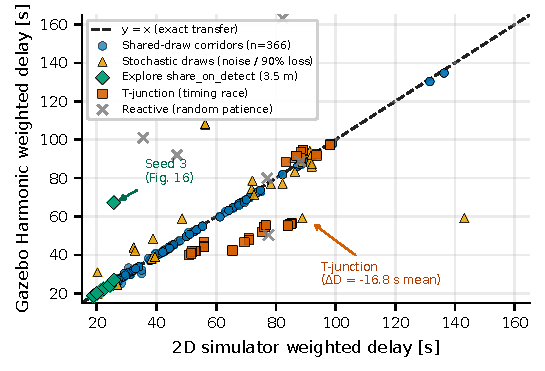
\includegraphics[width=\columnwidth]{Images/fig15_gazebo_scatter.pdf}
\caption{Paired Gazebo Harmonic versus 2D urgency-weighted delay across the 460-run main grid, showing tight clustering along $y=x$ for all 366 shared-draw corridor runs alongside isolated sim-to-3D divergence in T-junction timing races and $3.5$\,m \texttt{share\_on\_detect}.}
\label{fig:rq4_gz_scatter}
\end{figure}

Crucially, however, 3D Gazebo simulation revealed three physical and perceptual limits invisible in the 2D simulator.
\begin{enumerate}
\item \emph{Lidar peer-detection lag (\texttt{explore} and \texttt{hold\_for\_map}).} Whereas \texttt{sim2d} detects an oncoming robot immediately at $3.4$\,m inside the $3.5$\,m Lidar radius, Gazebo's wall-filtered \texttt{LaserScan} clustering ($0.35$\,m cluster distance matched within $2R_{\mathrm{sw}}=0.50$\,m of peer \texttt{STATE}) only registers an oncoming Waffle at $2.3$--$2.6$\,m separation on average. Consequently, even at $R_{\mathrm{det}}=3.5$\,m, \texttt{share\_on\_detect} delivered $0/6$ maps before decision time in Gazebo versus $6/6$ in 2D (Fig.~\ref{fig:rq4_gz_trace}), adding $+7.0$\,s of mean delay to \texttt{fixed\_priority} over the full-map Gazebo baseline ($+6.8$\,s over 2D). This mean is driven by a single run: on Seed~3, Robot~$B$ was sent to \texttt{room\_hi} ($+41.7$\,s), whereas in the other five runs the robots still chose \texttt{bay1} and Gazebo delay stayed within $0.2$\,s of the full-map baseline. Enabling \texttt{hold\_for\_map} (24 Gazebo runs) recovered the closer refuge (\texttt{bay1}) in $24/24$ runs, but peer detection occurred even closer ($1.10$--$1.18$\,m, waiting $4.7$\,s at $3.5$\,m and $9.5$\,s at $6.0$\,m), adding $+10.0$--$10.1$\,s over the full-map baseline. By then, Robot~$A$ ($6/6$) and Robot~$B$ ($5/6$) had already driven close enough to sense both bays directly, so holding worked in 3D by delaying the decision rather than by sharing maps. Including known bays in every \texttt{BID} (\texttt{share\_map}) avoids this lag entirely.
\item \emph{Branch-wall Lidar occlusion.} Early Gazebo T-junction runs showed that the $2.0$\,m side-branch walls block a parked branch robot's Lidar view of the main aisle (and exposed missing wall checks on room goals in 2D). Fusing fresh \texttt{STATE} positions into lane-clearance checks resolved this issue, meaning the final T-junction Gazebo runs serve as a post-fix verification rather than a blind transfer test.
\item \emph{Three-robot T-junction timing sensitivity ($\Delta D=-16.8$\,s).} Across all 36 T-junction runs, Gazebo accumulated $605.3$\,s less total delay than 2D ($-260.0$\,s across 18 exit runs and $-345.4$\,s across 18 turn-in runs). Event logs trace the exit gap (\cb\ $-264.7$\,s, \texttt{fixed\_priority} $+18.6$\,s, rulebook $-14.0$\,s) to a $\sim 20$\,s release-timing race. Under \cb\ in Gazebo, branch Robot~$S$ exits \texttt{bay1} slightly earlier while Robot~$A$ is still parked and slips past without triggering the second head-on conflict (or occasional $60$\,s proceed-timeout stall) seen in 2D, whereas under \texttt{fixed\_priority} and the rulebook, $S$ meets $A$ waiting in-lane and yields a second time ($4/4$ and $3/4$ runs). The larger turn-in offset ($9.5$--$28.9$\,s less delay per run and $0.4$--$6.4$\,s shorter makespan) remains an unexplained sim-to-3D timing gap, so exact T-junction delays cannot be predicted from 2D simulation alone.
\end{enumerate}

\begin{figure}[!t]\centering
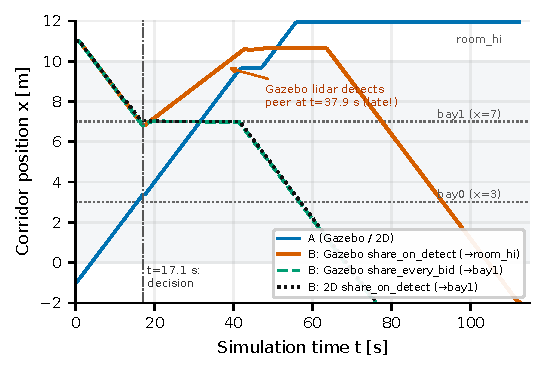
\includegraphics[width=\columnwidth]{Images/fig16_lidar_lag_trace.pdf}
\caption{Empirical spacetime trajectory $x(t)$ on Seed~3 ($R_{\mathrm{det}}=3.5$\,m): wall-filtered Gazebo Lidar clustering lags until $t=37.9$\,s, missing the $t=17.1$\,s decision window and sending $B$ to \texttt{room\_hi} instead of \texttt{bay1}.}
\label{fig:rq4_gz_trace}
\end{figure}
\section{Discussion, Limitations, and Future Work}\label{sec:disc}


\subsection{Synthesis and Fleet Engineering Selection Matrix}
Stepping back across RQ1--RQ4, resolving head-on single-lane encounters separates cleanly into two choices. The first is selecting a \emph{decision mechanism} based on fleet diversity, travel-time estimation accuracy, and whether robots belong to a single owner or competing vendors. The second is configuring the \emph{execution protocol} for wireless reliability, map completeness, and multi-robot geometry. Table~\ref{tab:guide} summarizes these quantitative findings into a practical selection guide for AMR system designers.

\begin{table*}[!t]\centering
\caption{Practitioner policy and protocol selection matrix distilled from $>50{,}000$ 2D and 496 ROS~2 / Gazebo episodes.}
\label{tab:guide}
{\footnotesize\renewcommand{\arraystretch}{1.22}\setlength{\tabcolsep}{6pt}
\begin{tabular}{@{}>{\raggedright\arraybackslash}p{0.195\textwidth}>{\raggedright\arraybackslash}p{0.205\textwidth}>{\raggedright\arraybackslash}p{0.240\textwidth}>{\raggedright\arraybackslash}p{0.290\textwidth}@{}}\toprule
Deployment Regime & Recommended Policy & Protocol Configuration & Empirical Basis \& Caveats \\\midrule
Homogeneous cooperative fleet; uncertain kinematics ($\sigma \ge 0.5$) & \texttt{rules\_proximity} (single-bay aisles) or \texttt{fixed\_priority}/\texttt{rules\_default} (multi-bay aisles); $\lambda=0.1$ credit where delay estimates exist & Periodic \texttt{STATE}/\texttt{BID}; \texttt{share\_map=true}; \texttt{commit} optional & Single bay: halves ID-priority excess ($3.1$ vs.\ $6.4$\,s) and matches noisy \cb\ at $\sigma\ge 0.5$; two bays: $5.6$ vs.\ $1.1$\,s for fixed priority. Credit rule (held-out $\lambda$) reaches $J=0.992$ for $+3.8\%$ delay ($+11.5\%$ at $\sigma=0.5$) \\\addlinespace[4.5pt]
Heterogeneous cooperative fleet (urgent / loaded / mixed speeds), $\sigma \le 0.35$ & Urgency-weighted \cb & \texttt{share\_map=true} on every \texttt{BID}; \texttt{refuge\_blocked} enabled & $0.04$\,s weighted excess ($98\%$ optimal match vs.\ $27.1$\,s fixed priority); ahead of both rulebooks up to $\sigma=0.35$, tied at $0.4$--$0.5$; avoids Lidar-lag penalty of \texttt{share\_on\_detect} \\\addlinespace[4.5pt]
Self-interested / multi-vendor robots sharing aisles & \texttt{clarke} (VCG pivot payment to operator ledger) & Authenticated IDs \& bay sets; audit joint bid scaling & $0.00$\,s unilateral misreport gain ($\le 0.02$\,s realized), with shared-snapshot types; generates a $24$--$37\%$ bank surplus (of realized delay) and $+4.9$\,s collusion incentive \\\addlinespace[4.5pt]
Convoys (2-vs.-1) \& branch junctions & Convoys: \texttt{fixed\_priority}; junctions: \cb; all with \texttt{make\_room}/\texttt{goal\_wait} & Fuse fresh \texttt{STATE} with Lidar for occluded junction lanes & \texttt{make\_room} \& \texttt{goal\_wait} restore $100\%$ completion; urgency rulebook is worst in convoys ($133.6$ vs.\ $90.3$\,s at $u_B=3$); model \emph{serial} follower clearance when $u_B \gg 1$ \\\addlinespace[4.5pt]
Legacy aisle without pull-in bays or off-lane staging queues & \texttt{reservation} (only if staging sits off exit path) & Corridor entry/exit \texttt{STATE} beacons & $100\%$ deadlock-free, but costs $+18.8$\,s excess when mid-aisle bays exist and staging blocks peer exit \\\bottomrule
\end{tabular}}
\end{table*}

Three broader lessons emerge from the experiments. First, \emph{broadcasting snapshots with attached bay lists outperforms complex handshakes}. Periodically broadcasting \texttt{BID} snapshots that include known and blocked bay IDs eliminates incomplete-map penalties at zero extra delay. By contrast, waiting for an explicit \texttt{commit} confirmation adds $3$--$4$\,s of delay under extreme packet loss without reducing collisions or deadlocks, and waiting for Lidar peer detection before sharing maps (\texttt{share\_on\_detect}) delivered no peer map before the decision in 3D Gazebo (0/6 runs) because of point-cloud clustering lag, sending one of the six runs to the far end room. Second, \emph{the benefit of cost bidding depends on matching the right fleet objective and having low estimation noise}. Minimizing unweighted delay when robots have different urgency weights wastes twice as much weighted time ($7.0$\,s) as a simple six-rule heuristic ($3.5$\,s), and, in the single-bay layout, bid estimation noise of $\sigma=0.5$ erases the advantage of \cb\ over a closest-refuge rulebook (which itself does not carry over to layouts with several bays). Third, \emph{simplified multi-robot delay models break down before 2D kinematics do}. In two-robot straight corridors, 2D excess delays transfer to 3D Gazebo within $1.0$\,s. However, three-robot convoys and T-junctions introduce sequential backing waits and branch-exit timing races that simple additive delay sums miss, requiring multi-robot timeline modeling and 3D physics validation.
\subsection{Limitations and Future Scope}
This study has several clear boundaries that point to directions for future work.
\begin{itemize}
\item \emph{Simulation-only evaluation and ground-truth localization.} All experiments were conducted in 2D and Gazebo Harmonic simulation (using 6 to 10 runs per Gazebo condition). Because the Gazebo nodes read ground-truth robot pose to isolate negotiation and Lidar perception, real-world factors such as AMCL or SLAM localization drift, wheel slip, and physical TurtleBot3 hardware dynamics remain to be tested.
\item \emph{Matched motion model and non-bid cheating.} Both \cb\ and \texttt{clarke} calculate bids using the simulator's true speed limits and bay coordinates. Systematic model errors (such as miscalibrated reverse speeds), strategic bay hiding, robot-ID spoofing during \texttt{commit} tie-breaks, mechanisms for redistributing accumulated VCG ledger credits, and voluntary participation incentives are not evaluated here.
\item \emph{Reactive baseline and theoretical liveness guarantees.} The only zero-communication baseline tested was centerline \texttt{reactive} backoff rather than continuous local planners such as ORCA, RVO, or CBFs. In addition, the protocol does not yet have a formal mathematical bound on how quickly temporary mutual yields ($14\%$--$24\%$ of runs under extreme packet loss) resolve, and the best forced yielder serves as a decision-level reference rather than a globally optimal continuous trajectory.
\item \emph{Simplified layouts and decision latency.} The T-junction approximates a side corridor as a $2$\,m-deep bay (leaving an unexplained $-345.4$\,s cumulative delay gap between Gazebo and 2D on the turn-in variant), \texttt{explore} discovers bays by geometric radius rather than full SLAM, the map-mismatch and blocked-bay sweeps use 10 seeds per condition, and the \texttt{learned} policy is a centralized tabular outcome classifier rather than deep MARL. Finally, every policy evaluated in this paper computes its decision in less than a millisecond of CPU time. Using large language or vision-language models (LLMs/VLMs)~\cite{marlin2024,gamechat2025,garg2024llm} as negotiators introduces multi-second inference delays while robots are still moving, along with decentralized disagreement failures that require dedicated asynchronous protocols and separate investigation.
\end{itemize}


\section{Conclusion}\label{sec:conc}
This paper presented an open dual-simulator benchmark for resolving head-on AMR encounters in narrow corridors with discrete pull-in bays, running the exact same 20\,Hz agent controller across more than 50,000 episodes in 2D simulation and 496 seed-paired runs in 3D ROS~2 Jazzy and Gazebo Harmonic. Communicating negotiation policies completely eliminate the $6.2\%$ deadlock rate and $\ge 3.6\times$ delay penalty of this zero-communication reactive design. Kinematic cost bidding matches the hindsight-yielder reference across symmetric corridors and reduces urgency-weighted excess delay for heterogeneous robots to $0.04$\,s, remaining superior to a simple closest-refuge rulebook in the single-bay layout until multiplicative bid estimation noise reaches $\sigma=0.5$ ($\approx0.45$ for heterogeneous fleets). For self-interested robots, Clarke-pivot (VCG) payments remove any single-robot gain from scaling cost bids, though at the expense of a $24\%$--$37\%$ ledger surplus (relative to realized delay) and vulnerability to joint bid shading. For cooperative fleets, a cumulative-delay fairness credit with $\lambda$ chosen on held-out sequences achieves a Jain fairness index of $0.992$ at $3.8\%$ extra delay. Periodically broadcasting snapshots maintains zero collisions even under $99\%$ packet loss, attaching bay lists removes incomplete-map penalties (tested up to $50\%$ loss), and the protocol reproduces $97.0\%$ of 2D yield decisions while matching straight-corridor excess delay within $1.0$\,s in 3D Gazebo, revealing practical transfer limits in Lidar peer clustering and three-robot junction timing. All source code, simulation worlds, study scripts, and per-episode datasets are publicly released at \url{https://github.com/briandeegan82/multi-agent-robots}.

\bibliographystyle{IEEEtran}
\bibliography{references}

% \begin{IEEEbiographynophoto}{Roshan George}
% Biography text here.
% \end{IEEEbiographynophoto}

% \begin{IEEEbiographynophoto}{Martin Glavin}
% Biography text here.
% \end{IEEEbiographynophoto}

% \begin{IEEEbiographynophoto}{Edward Jones}
% Biography text here.
% \end{IEEEbiographynophoto}

% \begin{IEEEbiographynophoto}{Brian Deegan}
% Biography text here.
% \end{IEEEbiographynophoto}

% \vfill

\end{document}
